\documentclass{article}
\usepackage{iclr2027_conference,times}
%%%%% NEW MATH DEFINITIONS %%%%%

\usepackage{amsmath,amsfonts,bm}

% Mark sections of captions for referring to divisions of figures
\newcommand{\figleft}{{\em (Left)}}
\newcommand{\figcenter}{{\em (Center)}}
\newcommand{\figright}{{\em (Right)}}
\newcommand{\figtop}{{\em (Top)}}
\newcommand{\figbottom}{{\em (Bottom)}}
\newcommand{\captiona}{{\em (a)}}
\newcommand{\captionb}{{\em (b)}}
\newcommand{\captionc}{{\em (c)}}
\newcommand{\captiond}{{\em (d)}}

% Highlight a newly defined term
\newcommand{\newterm}[1]{{\bf #1}}


% Figure reference, lower-case.
\def\figref#1{figure~\ref{#1}}
% Figure reference, capital. For start of sentence
\def\Figref#1{Figure~\ref{#1}}
\def\twofigref#1#2{figures \ref{#1} and \ref{#2}}
\def\quadfigref#1#2#3#4{figures \ref{#1}, \ref{#2}, \ref{#3} and \ref{#4}}
% Section reference, lower-case.
\def\secref#1{section~\ref{#1}}
% Section reference, capital.
\def\Secref#1{Section~\ref{#1}}
% Reference to two sections.
\def\twosecrefs#1#2{sections \ref{#1} and \ref{#2}}
% Reference to three sections.
\def\secrefs#1#2#3{sections \ref{#1}, \ref{#2} and \ref{#3}}
% Reference to an equation, lower-case.
\def\eqref#1{equation~\ref{#1}}
% Reference to an equation, upper case
\def\Eqref#1{Equation~\ref{#1}}
% A raw reference to an equation---avoid using if possible
\def\plaineqref#1{\ref{#1}}
% Reference to a chapter, lower-case.
\def\chapref#1{chapter~\ref{#1}}
% Reference to an equation, upper case.
\def\Chapref#1{Chapter~\ref{#1}}
% Reference to a range of chapters
\def\rangechapref#1#2{chapters\ref{#1}--\ref{#2}}
% Reference to an algorithm, lower-case.
\def\algref#1{algorithm~\ref{#1}}
% Reference to an algorithm, upper case.
\def\Algref#1{Algorithm~\ref{#1}}
\def\twoalgref#1#2{algorithms \ref{#1} and \ref{#2}}
\def\Twoalgref#1#2{Algorithms \ref{#1} and \ref{#2}}
% Reference to a part, lower case
\def\partref#1{part~\ref{#1}}
% Reference to a part, upper case
\def\Partref#1{Part~\ref{#1}}
\def\twopartref#1#2{parts \ref{#1} and \ref{#2}}

\def\ceil#1{\lceil #1 \rceil}
\def\floor#1{\lfloor #1 \rfloor}
\def\1{\bm{1}}
\newcommand{\train}{\mathcal{D}}
\newcommand{\valid}{\mathcal{D_{\mathrm{valid}}}}
\newcommand{\test}{\mathcal{D_{\mathrm{test}}}}

\def\eps{{\epsilon}}


% Random variables
\def\reta{{\textnormal{$\eta$}}}
\def\ra{{\textnormal{a}}}
\def\rb{{\textnormal{b}}}
\def\rc{{\textnormal{c}}}
\def\rd{{\textnormal{d}}}
\def\re{{\textnormal{e}}}
\def\rf{{\textnormal{f}}}
\def\rg{{\textnormal{g}}}
\def\rh{{\textnormal{h}}}
\def\ri{{\textnormal{i}}}
\def\rj{{\textnormal{j}}}
\def\rk{{\textnormal{k}}}
\def\rl{{\textnormal{l}}}
% rm is already a command, just don't name any random variables m
\def\rn{{\textnormal{n}}}
\def\ro{{\textnormal{o}}}
\def\rp{{\textnormal{p}}}
\def\rq{{\textnormal{q}}}
\def\rr{{\textnormal{r}}}
\def\rs{{\textnormal{s}}}
\def\rt{{\textnormal{t}}}
\def\ru{{\textnormal{u}}}
\def\rv{{\textnormal{v}}}
\def\rw{{\textnormal{w}}}
\def\rx{{\textnormal{x}}}
\def\ry{{\textnormal{y}}}
\def\rz{{\textnormal{z}}}

% Random vectors
\def\rvepsilon{{\mathbf{\epsilon}}}
\def\rvtheta{{\mathbf{\theta}}}
\def\rva{{\mathbf{a}}}
\def\rvb{{\mathbf{b}}}
\def\rvc{{\mathbf{c}}}
\def\rvd{{\mathbf{d}}}
\def\rve{{\mathbf{e}}}
\def\rvf{{\mathbf{f}}}
\def\rvg{{\mathbf{g}}}
\def\rvh{{\mathbf{h}}}
\def\rvu{{\mathbf{i}}}
\def\rvj{{\mathbf{j}}}
\def\rvk{{\mathbf{k}}}
\def\rvl{{\mathbf{l}}}
\def\rvm{{\mathbf{m}}}
\def\rvn{{\mathbf{n}}}
\def\rvo{{\mathbf{o}}}
\def\rvp{{\mathbf{p}}}
\def\rvq{{\mathbf{q}}}
\def\rvr{{\mathbf{r}}}
\def\rvs{{\mathbf{s}}}
\def\rvt{{\mathbf{t}}}
\def\rvu{{\mathbf{u}}}
\def\rvv{{\mathbf{v}}}
\def\rvw{{\mathbf{w}}}
\def\rvx{{\mathbf{x}}}
\def\rvy{{\mathbf{y}}}
\def\rvz{{\mathbf{z}}}

% Elements of random vectors
\def\erva{{\textnormal{a}}}
\def\ervb{{\textnormal{b}}}
\def\ervc{{\textnormal{c}}}
\def\ervd{{\textnormal{d}}}
\def\erve{{\textnormal{e}}}
\def\ervf{{\textnormal{f}}}
\def\ervg{{\textnormal{g}}}
\def\ervh{{\textnormal{h}}}
\def\ervi{{\textnormal{i}}}
\def\ervj{{\textnormal{j}}}
\def\ervk{{\textnormal{k}}}
\def\ervl{{\textnormal{l}}}
\def\ervm{{\textnormal{m}}}
\def\ervn{{\textnormal{n}}}
\def\ervo{{\textnormal{o}}}
\def\ervp{{\textnormal{p}}}
\def\ervq{{\textnormal{q}}}
\def\ervr{{\textnormal{r}}}
\def\ervs{{\textnormal{s}}}
\def\ervt{{\textnormal{t}}}
\def\ervu{{\textnormal{u}}}
\def\ervv{{\textnormal{v}}}
\def\ervw{{\textnormal{w}}}
\def\ervx{{\textnormal{x}}}
\def\ervy{{\textnormal{y}}}
\def\ervz{{\textnormal{z}}}

% Random matrices
\def\rmA{{\mathbf{A}}}
\def\rmB{{\mathbf{B}}}
\def\rmC{{\mathbf{C}}}
\def\rmD{{\mathbf{D}}}
\def\rmE{{\mathbf{E}}}
\def\rmF{{\mathbf{F}}}
\def\rmG{{\mathbf{G}}}
\def\rmH{{\mathbf{H}}}
\def\rmI{{\mathbf{I}}}
\def\rmJ{{\mathbf{J}}}
\def\rmK{{\mathbf{K}}}
\def\rmL{{\mathbf{L}}}
\def\rmM{{\mathbf{M}}}
\def\rmN{{\mathbf{N}}}
\def\rmO{{\mathbf{O}}}
\def\rmP{{\mathbf{P}}}
\def\rmQ{{\mathbf{Q}}}
\def\rmR{{\mathbf{R}}}
\def\rmS{{\mathbf{S}}}
\def\rmT{{\mathbf{T}}}
\def\rmU{{\mathbf{U}}}
\def\rmV{{\mathbf{V}}}
\def\rmW{{\mathbf{W}}}
\def\rmX{{\mathbf{X}}}
\def\rmY{{\mathbf{Y}}}
\def\rmZ{{\mathbf{Z}}}

% Elements of random matrices
\def\ermA{{\textnormal{A}}}
\def\ermB{{\textnormal{B}}}
\def\ermC{{\textnormal{C}}}
\def\ermD{{\textnormal{D}}}
\def\ermE{{\textnormal{E}}}
\def\ermF{{\textnormal{F}}}
\def\ermG{{\textnormal{G}}}
\def\ermH{{\textnormal{H}}}
\def\ermI{{\textnormal{I}}}
\def\ermJ{{\textnormal{J}}}
\def\ermK{{\textnormal{K}}}
\def\ermL{{\textnormal{L}}}
\def\ermM{{\textnormal{M}}}
\def\ermN{{\textnormal{N}}}
\def\ermO{{\textnormal{O}}}
\def\ermP{{\textnormal{P}}}
\def\ermQ{{\textnormal{Q}}}
\def\ermR{{\textnormal{R}}}
\def\ermS{{\textnormal{S}}}
\def\ermT{{\textnormal{T}}}
\def\ermU{{\textnormal{U}}}
\def\ermV{{\textnormal{V}}}
\def\ermW{{\textnormal{W}}}
\def\ermX{{\textnormal{X}}}
\def\ermY{{\textnormal{Y}}}
\def\ermZ{{\textnormal{Z}}}

% Vectors
\def\vzero{{\bm{0}}}
\def\vone{{\bm{1}}}
\def\vmu{{\bm{\mu}}}
\def\vtheta{{\bm{\theta}}}
\def\va{{\bm{a}}}
\def\vb{{\bm{b}}}
\def\vc{{\bm{c}}}
\def\vd{{\bm{d}}}
\def\ve{{\bm{e}}}
\def\vf{{\bm{f}}}
\def\vg{{\bm{g}}}
\def\vh{{\bm{h}}}
\def\vi{{\bm{i}}}
\def\vj{{\bm{j}}}
\def\vk{{\bm{k}}}
\def\vl{{\bm{l}}}
\def\vm{{\bm{m}}}
\def\vn{{\bm{n}}}
\def\vo{{\bm{o}}}
\def\vp{{\bm{p}}}
\def\vq{{\bm{q}}}
\def\vr{{\bm{r}}}
\def\vs{{\bm{s}}}
\def\vt{{\bm{t}}}
\def\vu{{\bm{u}}}
\def\vv{{\bm{v}}}
\def\vw{{\bm{w}}}
\def\vx{{\bm{x}}}
\def\vy{{\bm{y}}}
\def\vz{{\bm{z}}}

% Elements of vectors
\def\evalpha{{\alpha}}
\def\evbeta{{\beta}}
\def\evepsilon{{\epsilon}}
\def\evlambda{{\lambda}}
\def\evomega{{\omega}}
\def\evmu{{\mu}}
\def\evpsi{{\psi}}
\def\evsigma{{\sigma}}
\def\evtheta{{\theta}}
\def\eva{{a}}
\def\evb{{b}}
\def\evc{{c}}
\def\evd{{d}}
\def\eve{{e}}
\def\evf{{f}}
\def\evg{{g}}
\def\evh{{h}}
\def\evi{{i}}
\def\evj{{j}}
\def\evk{{k}}
\def\evl{{l}}
\def\evm{{m}}
\def\evn{{n}}
\def\evo{{o}}
\def\evp{{p}}
\def\evq{{q}}
\def\evr{{r}}
\def\evs{{s}}
\def\evt{{t}}
\def\evu{{u}}
\def\evv{{v}}
\def\evw{{w}}
\def\evx{{x}}
\def\evy{{y}}
\def\evz{{z}}

% Matrix
\def\mA{{\bm{A}}}
\def\mB{{\bm{B}}}
\def\mC{{\bm{C}}}
\def\mD{{\bm{D}}}
\def\mE{{\bm{E}}}
\def\mF{{\bm{F}}}
\def\mG{{\bm{G}}}
\def\mH{{\bm{H}}}
\def\mI{{\bm{I}}}
\def\mJ{{\bm{J}}}
\def\mK{{\bm{K}}}
\def\mL{{\bm{L}}}
\def\mM{{\bm{M}}}
\def\mN{{\bm{N}}}
\def\mO{{\bm{O}}}
\def\mP{{\bm{P}}}
\def\mQ{{\bm{Q}}}
\def\mR{{\bm{R}}}
\def\mS{{\bm{S}}}
\def\mT{{\bm{T}}}
\def\mU{{\bm{U}}}
\def\mV{{\bm{V}}}
\def\mW{{\bm{W}}}
\def\mX{{\bm{X}}}
\def\mY{{\bm{Y}}}
\def\mZ{{\bm{Z}}}
\def\mBeta{{\bm{\beta}}}
\def\mPhi{{\bm{\Phi}}}
\def\mLambda{{\bm{\Lambda}}}
\def\mSigma{{\bm{\Sigma}}}

% Tensor
\DeclareMathAlphabet{\mathsfit}{\encodingdefault}{\sfdefault}{m}{sl}
\SetMathAlphabet{\mathsfit}{bold}{\encodingdefault}{\sfdefault}{bx}{n}
\newcommand{\tens}[1]{\bm{\mathsfit{#1}}}
\def\tA{{\tens{A}}}
\def\tB{{\tens{B}}}
\def\tC{{\tens{C}}}
\def\tD{{\tens{D}}}
\def\tE{{\tens{E}}}
\def\tF{{\tens{F}}}
\def\tG{{\tens{G}}}
\def\tH{{\tens{H}}}
\def\tI{{\tens{I}}}
\def\tJ{{\tens{J}}}
\def\tK{{\tens{K}}}
\def\tL{{\tens{L}}}
\def\tM{{\tens{M}}}
\def\tN{{\tens{N}}}
\def\tO{{\tens{O}}}
\def\tP{{\tens{P}}}
\def\tQ{{\tens{Q}}}
\def\tR{{\tens{R}}}
\def\tS{{\tens{S}}}
\def\tT{{\tens{T}}}
\def\tU{{\tens{U}}}
\def\tV{{\tens{V}}}
\def\tW{{\tens{W}}}
\def\tX{{\tens{X}}}
\def\tY{{\tens{Y}}}
\def\tZ{{\tens{Z}}}


% Graph
\def\gA{{\mathcal{A}}}
\def\gB{{\mathcal{B}}}
\def\gC{{\mathcal{C}}}
\def\gD{{\mathcal{D}}}
\def\gE{{\mathcal{E}}}
\def\gF{{\mathcal{F}}}
\def\gG{{\mathcal{G}}}
\def\gH{{\mathcal{H}}}
\def\gI{{\mathcal{I}}}
\def\gJ{{\mathcal{J}}}
\def\gK{{\mathcal{K}}}
\def\gL{{\mathcal{L}}}
\def\gM{{\mathcal{M}}}
\def\gN{{\mathcal{N}}}
\def\gO{{\mathcal{O}}}
\def\gP{{\mathcal{P}}}
\def\gQ{{\mathcal{Q}}}
\def\gR{{\mathcal{R}}}
\def\gS{{\mathcal{S}}}
\def\gT{{\mathcal{T}}}
\def\gU{{\mathcal{U}}}
\def\gV{{\mathcal{V}}}
\def\gW{{\mathcal{W}}}
\def\gX{{\mathcal{X}}}
\def\gY{{\mathcal{Y}}}
\def\gZ{{\mathcal{Z}}}

% Sets
\def\sA{{\mathbb{A}}}
\def\sB{{\mathbb{B}}}
\def\sC{{\mathbb{C}}}
\def\sD{{\mathbb{D}}}
% Don't use a set called E, because this would be the same as our symbol
% for expectation.
\def\sF{{\mathbb{F}}}
\def\sG{{\mathbb{G}}}
\def\sH{{\mathbb{H}}}
\def\sI{{\mathbb{I}}}
\def\sJ{{\mathbb{J}}}
\def\sK{{\mathbb{K}}}
\def\sL{{\mathbb{L}}}
\def\sM{{\mathbb{M}}}
\def\sN{{\mathbb{N}}}
\def\sO{{\mathbb{O}}}
\def\sP{{\mathbb{P}}}
\def\sQ{{\mathbb{Q}}}
\def\sR{{\mathbb{R}}}
\def\sS{{\mathbb{S}}}
\def\sT{{\mathbb{T}}}
\def\sU{{\mathbb{U}}}
\def\sV{{\mathbb{V}}}
\def\sW{{\mathbb{W}}}
\def\sX{{\mathbb{X}}}
\def\sY{{\mathbb{Y}}}
\def\sZ{{\mathbb{Z}}}

% Entries of a matrix
\def\emLambda{{\Lambda}}
\def\emA{{A}}
\def\emB{{B}}
\def\emC{{C}}
\def\emD{{D}}
\def\emE{{E}}
\def\emF{{F}}
\def\emG{{G}}
\def\emH{{H}}
\def\emI{{I}}
\def\emJ{{J}}
\def\emK{{K}}
\def\emL{{L}}
\def\emM{{M}}
\def\emN{{N}}
\def\emO{{O}}
\def\emP{{P}}
\def\emQ{{Q}}
\def\emR{{R}}
\def\emS{{S}}
\def\emT{{T}}
\def\emU{{U}}
\def\emV{{V}}
\def\emW{{W}}
\def\emX{{X}}
\def\emY{{Y}}
\def\emZ{{Z}}
\def\emSigma{{\Sigma}}

% entries of a tensor
% Same font as tensor, without \bm wrapper
\newcommand{\etens}[1]{\mathsfit{#1}}
\def\etLambda{{\etens{\Lambda}}}
\def\etA{{\etens{A}}}
\def\etB{{\etens{B}}}
\def\etC{{\etens{C}}}
\def\etD{{\etens{D}}}
\def\etE{{\etens{E}}}
\def\etF{{\etens{F}}}
\def\etG{{\etens{G}}}
\def\etH{{\etens{H}}}
\def\etI{{\etens{I}}}
\def\etJ{{\etens{J}}}
\def\etK{{\etens{K}}}
\def\etL{{\etens{L}}}
\def\etM{{\etens{M}}}
\def\etN{{\etens{N}}}
\def\etO{{\etens{O}}}
\def\etP{{\etens{P}}}
\def\etQ{{\etens{Q}}}
\def\etR{{\etens{R}}}
\def\etS{{\etens{S}}}
\def\etT{{\etens{T}}}
\def\etU{{\etens{U}}}
\def\etV{{\etens{V}}}
\def\etW{{\etens{W}}}
\def\etX{{\etens{X}}}
\def\etY{{\etens{Y}}}
\def\etZ{{\etens{Z}}}

% The true underlying data generating distribution
\newcommand{\pdata}{p_{\rm{data}}}
% The empirical distribution defined by the training set
\newcommand{\ptrain}{\hat{p}_{\rm{data}}}
\newcommand{\Ptrain}{\hat{P}_{\rm{data}}}
% The model distribution
\newcommand{\pmodel}{p_{\rm{model}}}
\newcommand{\Pmodel}{P_{\rm{model}}}
\newcommand{\ptildemodel}{\tilde{p}_{\rm{model}}}
% Stochastic autoencoder distributions
\newcommand{\pencode}{p_{\rm{encoder}}}
\newcommand{\pdecode}{p_{\rm{decoder}}}
\newcommand{\precons}{p_{\rm{reconstruct}}}

\newcommand{\laplace}{\mathrm{Laplace}} % Laplace distribution

\newcommand{\E}{\mathbb{E}}
\newcommand{\Ls}{\mathcal{L}}
\newcommand{\R}{\mathbb{R}}
\newcommand{\emp}{\tilde{p}}
\newcommand{\lr}{\alpha}
\newcommand{\reg}{\lambda}
\newcommand{\rect}{\mathrm{rectifier}}
\newcommand{\softmax}{\mathrm{softmax}}
\newcommand{\sigmoid}{\sigma}
\newcommand{\softplus}{\zeta}
\newcommand{\KL}{D_{\mathrm{KL}}}
\newcommand{\Var}{\mathrm{Var}}
\newcommand{\standarderror}{\mathrm{SE}}
\newcommand{\Cov}{\mathrm{Cov}}
% Wolfram Mathworld says $L^2$ is for function spaces and $\ell^2$ is for vectors
% But then they seem to use $L^2$ for vectors throughout the site, and so does
% wikipedia.
\newcommand{\normlzero}{L^0}
\newcommand{\normlone}{L^1}
\newcommand{\normltwo}{L^2}
\newcommand{\normlp}{L^p}
\newcommand{\normmax}{L^\infty}

\newcommand{\parents}{Pa} % See usage in notation.tex. Chosen to match Daphne's book.

\DeclareMathOperator*{\argmax}{arg\,max}
\DeclareMathOperator*{\argmin}{arg\,min}

\DeclareMathOperator{\sign}{sign}
\DeclareMathOperator{\Tr}{Tr}
\let\ab\allowbreak


\usepackage{url}
\usepackage{booktabs}
\usepackage{graphicx}
\usepackage{amsmath,amssymb}
\usepackage{enumitem}
\usepackage{float}
\usepackage{wrapfig}
\usepackage{needspace}
\usepackage{multirow}
\usepackage{xcolor}
\usepackage{algorithm}
\usepackage{algorithmic}
\usepackage{hyperref}
\hypersetup{hidelinks}

\providecommand{\pym}[1]{}
\newcommand{\triage}{\textsc{Triage}\,}
\newcommand{\method}{\textsc{Triage-PiEvo}\,}
\newcommand{\pievo}{\textsc{PiEvo}\,}
\newcommand{\revise}{\mathsf{revise}\,}
\newcommand{\retain}{\mathsf{retain}\,}
\newcommand{\verify}{\mathsf{verify}\,}

\title{Triage-PiEvo: Source-Aware Anomaly Diagnosis before Principle Revision}

% Anonymous submission. Do not reveal author identities or repository links.
\author{Anonymous Authors}

\begin{document}

\maketitle

\begin{abstract}
Principle-evolving scientific agents can move beyond incomplete initial hypotheses by revising the principles that guide discovery. Yet a large residual is ambiguous: it may reveal a new mechanism, or arise from evaluator corruption, surrogate mismatch, or a local effect that fails to generalize. We introduce \triage{}, a source-aware evidence-admission layer that separates anomaly detection from authorization to revise persistent scientific state. \triage{} maintains distinct primary and verification histories, updates channel reliability from reconciliation outcomes, and keeps a proposed principle provisional until it receives independent held-out support; contradictory held-out evidence retracts the principle and its descendants. We instantiate this protocol in \method{}, pairing \triage{} with an outcome-blind Active Flow Expansion portfolio for exploitation, frontier expansion, and mechanism-discriminating probes. Across four matched discovery tasks and three backbone LLMs, \method{} achieves the highest average solution quality and area under the optimization curve for each backbone, reaching $79.63$--$83.37$ average solution quality and improving over the strongest baseline for each backbone by $7.5$ to $11.8$ points. A component study separates the two contributions: search expansion recovers clean-task quality, whereas the admission gate is decisive under unreliable feedback. In controlled corruption, hidden-source, reversal, and proxy-exploitation studies, the gate reduces corrupted-evidence admission from $1.0$ to $0.0$, rejects the tested non-generalizing artifacts without missing the tested true mechanism, and enables retraction after reversal. The results show that an observation can be useful for directing search before it is reliable enough to justify persistent principle revision.
\end{abstract}

\section{Introduction}

\begin{wrapfigure}[18]{r}{0.38\textwidth}
    \vspace{-12pt}
    \centering
    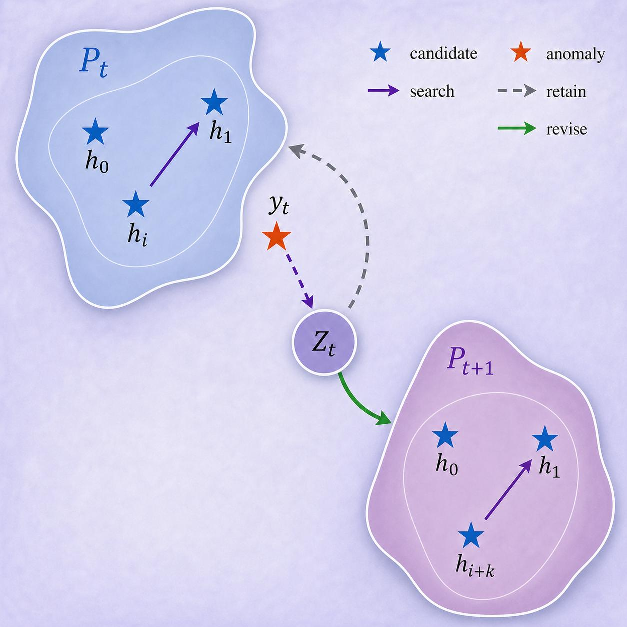
\includegraphics[width=0.88\linewidth]{figures/triage-overview.pdf}
    \vspace{-5pt}
    \caption{\textbf{Source-aware triage (schematic).} Latent source $Z_t$ mediates the verified retain-or-revise decision.}
    \label{fig:triage-overview}
    \vspace{-12pt}
\end{wrapfigure}

% P1 Background: field capability -> task narrowing -> field-level bottleneck.
Autonomous scientific agents now automate scientific research within a single closed loop~\citep{lu2024aiscientist,yamada2025aiscientistv2workshoplevelautomated,schmidgall2025agentlaboratory,gottweis2025aicoscientist}. 
On the premise that true knowledge often lies outside the initial hypothesis space, principle-evolution agents~\citep{pu2026pievo, pu2026piflowprincipleawarescientificdiscovery} make every anomaly a decision in this loop: steer hypothesis search, or rewrite the persisted theory and explanation.

% P2 Prior response -> retained constraint -> diagnostic close.
While surprise-driven revision~\citep{pu2026pievo} lets agents escape their initial hypothesis space, it treats the observation's reliability as given. Consequently, the decision rests on a signal that cannot discriminate---the residual magnitude of surprisal may stem from corrupted measurements or surrogate misspecification; thresholding it therefore trades false revisions against missed theory blindly.
Nor do existing methods cover this gap: verification loops critique transient responses rather than persisted theory~\citep{shinn2023reflexion,madaan2023selfrefine,gou2023critic,dhuliawala2024chainverification}, and self-correction without external evidence is unreliable~\citep{huang2023cannotselfcorrect,kamoi2024selfcorrection}. 
Accordingly, community evaluations find that auto-research agents produce extensive artifacts yet seldom revise their internal theory under contradictory evidence~\citep{riosgarcia2026aiscientistsproduceresults,kirgis2026openendedresearch}. 
This rigidity leads to significant inefficiencies: \emph{anomalies are read as evidence of science, corrupted feedback enters trusted scientific state}.

% P3 Challenge decomposition.
These limitations reduce to three challenges: (a) one anomaly score has \textbf{source ambiguity} that cannot tell a new mechanism from corrupted or misspecified evaluations; (b) the \textbf{role conflation} of one history serves both search and principle acceptance, so unreliable observations can rewrite trusted principles; and (c) the \textbf{revision irreversibility} that accepted principles cannot be retracted under contradictory evidence.

% P4 Method bridge: conceptual reframing and feedback loop, no equations.
To bridge this gap, we propose \textbf{\triage}, an evidence-admission layer that decouples anomaly detection from principle revision. 
\triage infers over a latent source variable for each anomaly and routes evidence along two paths with distinct standards: search outcomes accumulate in a primary history that steers candidate selection, while verification records---same-channel repeats, cross-channel checks, held-out probes---are logged separately and update per-channel reliability estimates. A proposed principle is accepted only after independent held-out support; contradictory held-out evidence retracts it and its descendants. An observation can thus remain search-active while its scientific interpretation stays provisional. We instantiate this protocol in \textbf{\method{}}, which pairs \triage{} with an outcome-blind Active Flow Expansion (AFE) portfolio: the portfolio allocates the evaluation budget across exploitation, frontier expansion, and mechanism-discriminating probes, while the gate alone decides which evidence may alter principle state.

% P5 Evidence preview: indexed findings in challenge order.
We evaluate \method on four discovery tasks under three backbone LLMs.
Empirical results demonstrate that \textbf{\method}: 
(a) \textbf{attains the highest performance}, raising average solution quality from \pievo's $62.87$--$70.35$\% to $79.63$--$83.37$\%; 
(b) \textbf{admits no corrupted observations} where gate-off variants admit every one (admission rate $0.000$ vs.\ $1.000$) under transient and persistent evaluator corruption;
(c) \textbf{cuts false expansions} on noise, surrogate failure, and non-generalizing local artifacts from $1.0$ to $0.0$ without missing any true mechanism, and backtracks to the correct state after mechanism reversal; and
(d) \textbf{admits no exploit-region evidence} under proxy exploitation, raising held-out score by $0.209$ at only $+13.6\%$ runtime over \pievo{}.

In summary, our contributions are:
\begin{enumerate}[nosep, leftmargin=12pt]
  \item[(a)] We introduce \textbf{evidence admission} as the decision layer of principle-evolving agents: anomalies are attributed to latent sources, and revision is governed by asymmetric costs of false revision versus missed mechanism, replacing surprise thresholding as the trigger for changing scientific state.
  \item[(b)] We propose \textbf{\method{}}, which realizes this layer through per-channel trust estimation, a proposed--provisional--accepted--retracted principle lifecycle gated by independent held-out support, and an outcome-blind search portfolio, with all admission thresholds fixed before evaluation.
  \item[(c)] We provide \textbf{evidence separating search from revision}: across four tasks and three backbones, \method{} raises average discovery quality, and controlled corruption, hidden-source, reversal, and proxy-exploitation studies show that the gate rejects unreliable evidence without rejecting genuine mechanisms.
\end{enumerate}

\section{Related Work}
\label{sec:related}

\subsection{Autonomous Scientific Agents and Evolving State}
Scientific agents automate growing shares of the research cycle, from end-to-end paper production and multi-stage pipelines~\citep{lu2024aiscientist,yamada2025aiscientistv2workshoplevelautomated,tang2025airesearcherautonomousscientificinnovation,schmidgall2025agentlaboratory,gottweis2025aicoscientist} to tool-coupled domain execution and closed-loop laboratory discovery~\citep{bran2024chemcrow,boiko2023autonomouschemical,ruan2024llmrdf,yang2024moosechem,ghafarollahi2024sciagents,ding2025scitoolagent,ghareeb2026robin,narayanan2024aviary,laurent2024labbench,mitchener2025bixbench,skarlinski2024paperqa2,mitchener2025kosmos}. What persists between iterations there is an artifact, not a revisable scientific account. A narrower line makes the internal state editable: \pievo{} and PiFlow expand a principle space on conflicting observations~\citep{pu2026pievo,pu2026piflowprincipleawarescientificdiscovery}, ATLAS selects mechanism-discriminating experiments~\citep{elteto2026atlas}, self-revising frameworks log regime changes~\citep{wang2026selfrevising}, and evolving architectures such as EvoMaster~\citep{zhu2026evomaster} and ADMET-EvO~\citep{zhou2026admetevo} pursue cumulative adaptation across tasks, with agentic laboratory world models unifying hypothesis generation and state tracking~\citep{fu2026agenticlab}. Editable state is also corruptible: without explicit evidence admission, anomalous or corrupted feedback rewrites persistent principles directly~\citep{riosgarcia2026aiscientistsproduceresults,kirgis2026openendedresearch}. \triage{} separates the history that steers search from the evidence authorized to alter scientific state.

\subsection{Active Experimentation under Heterogeneous Sources}
In active learning and Bayesian optimization, one line decides where to spend evaluations~\citep{mackay1992information,houlsby2011bayesianactivelearningclassification}, constraining exploration for safety~\citep{sui2015safeopt} or scalability~\citep{eriksson2019turbo}. Another exploits heterogeneous costs, fidelities, and failure rates across sources~\citep{swersky2013multitask,kandasamy2017multifidelitybayesianoptimisationcontinuous,poloczek2017multiinformation,ghoreishi2018multinformation}, extending to unreliable channels~\citep{mikkola2023multifidelity,fan2024inputdependentmfbo}, quality-controlled loops~\citep{harris2025activeoversightqualitycontrol}, and out-of-distribution expansion~\citep{desanti2026actflow}. Both decide which observation to acquire \emph{before} it is run, so an anomalous outcome inherits whatever reliability the acquisition rule assumed. The difference is in what the decision protects: multi-source methods weight a noisy source inside a regression model, while the object at risk here is a persistent principle that a single admitted artifact can corrupt for the rest of the run. Our AFE portfolio takes the acquisition-side view for candidate generation; \triage{} makes the post-observation decision of whether an anomaly may update that principle.

\subsection{Verification, Provenance, and Agent Monitoring}
In agent systems, verification targets transient outputs through feedback recycling~\citep{yao2023reactsynergizingreasoningacting,shinn2023reflexion,madaan2023selfrefine}, tool-based checking~\citep{gou2023critic}, independent verification questions~\citep{dhuliawala2024chainverification}, and evidence accumulation~\citep{zhang2026glean}, though self-correction without external evidence is unreliable~\citep{huang2023cannotselfcorrect,kamoi2024selfcorrection}. Related work argues for monitoring agentic systems before trusting them~\citep{boston2026monitoring} and for immutable provenance trails over agent-generated artifacts~\citep{liu2026lasthuman}, while Sibyl~\citep{rangelov2026sibyl} uses temporal backtesting as held-out evidence. \triage{} carries these provenance and monitoring ideas to persistent principles: same-source agreement keeps observations search-active, acceptance requires independent held-out support, and contradictory held-out evidence forces retraction.

\begin{figure*}[t]
    \centering
    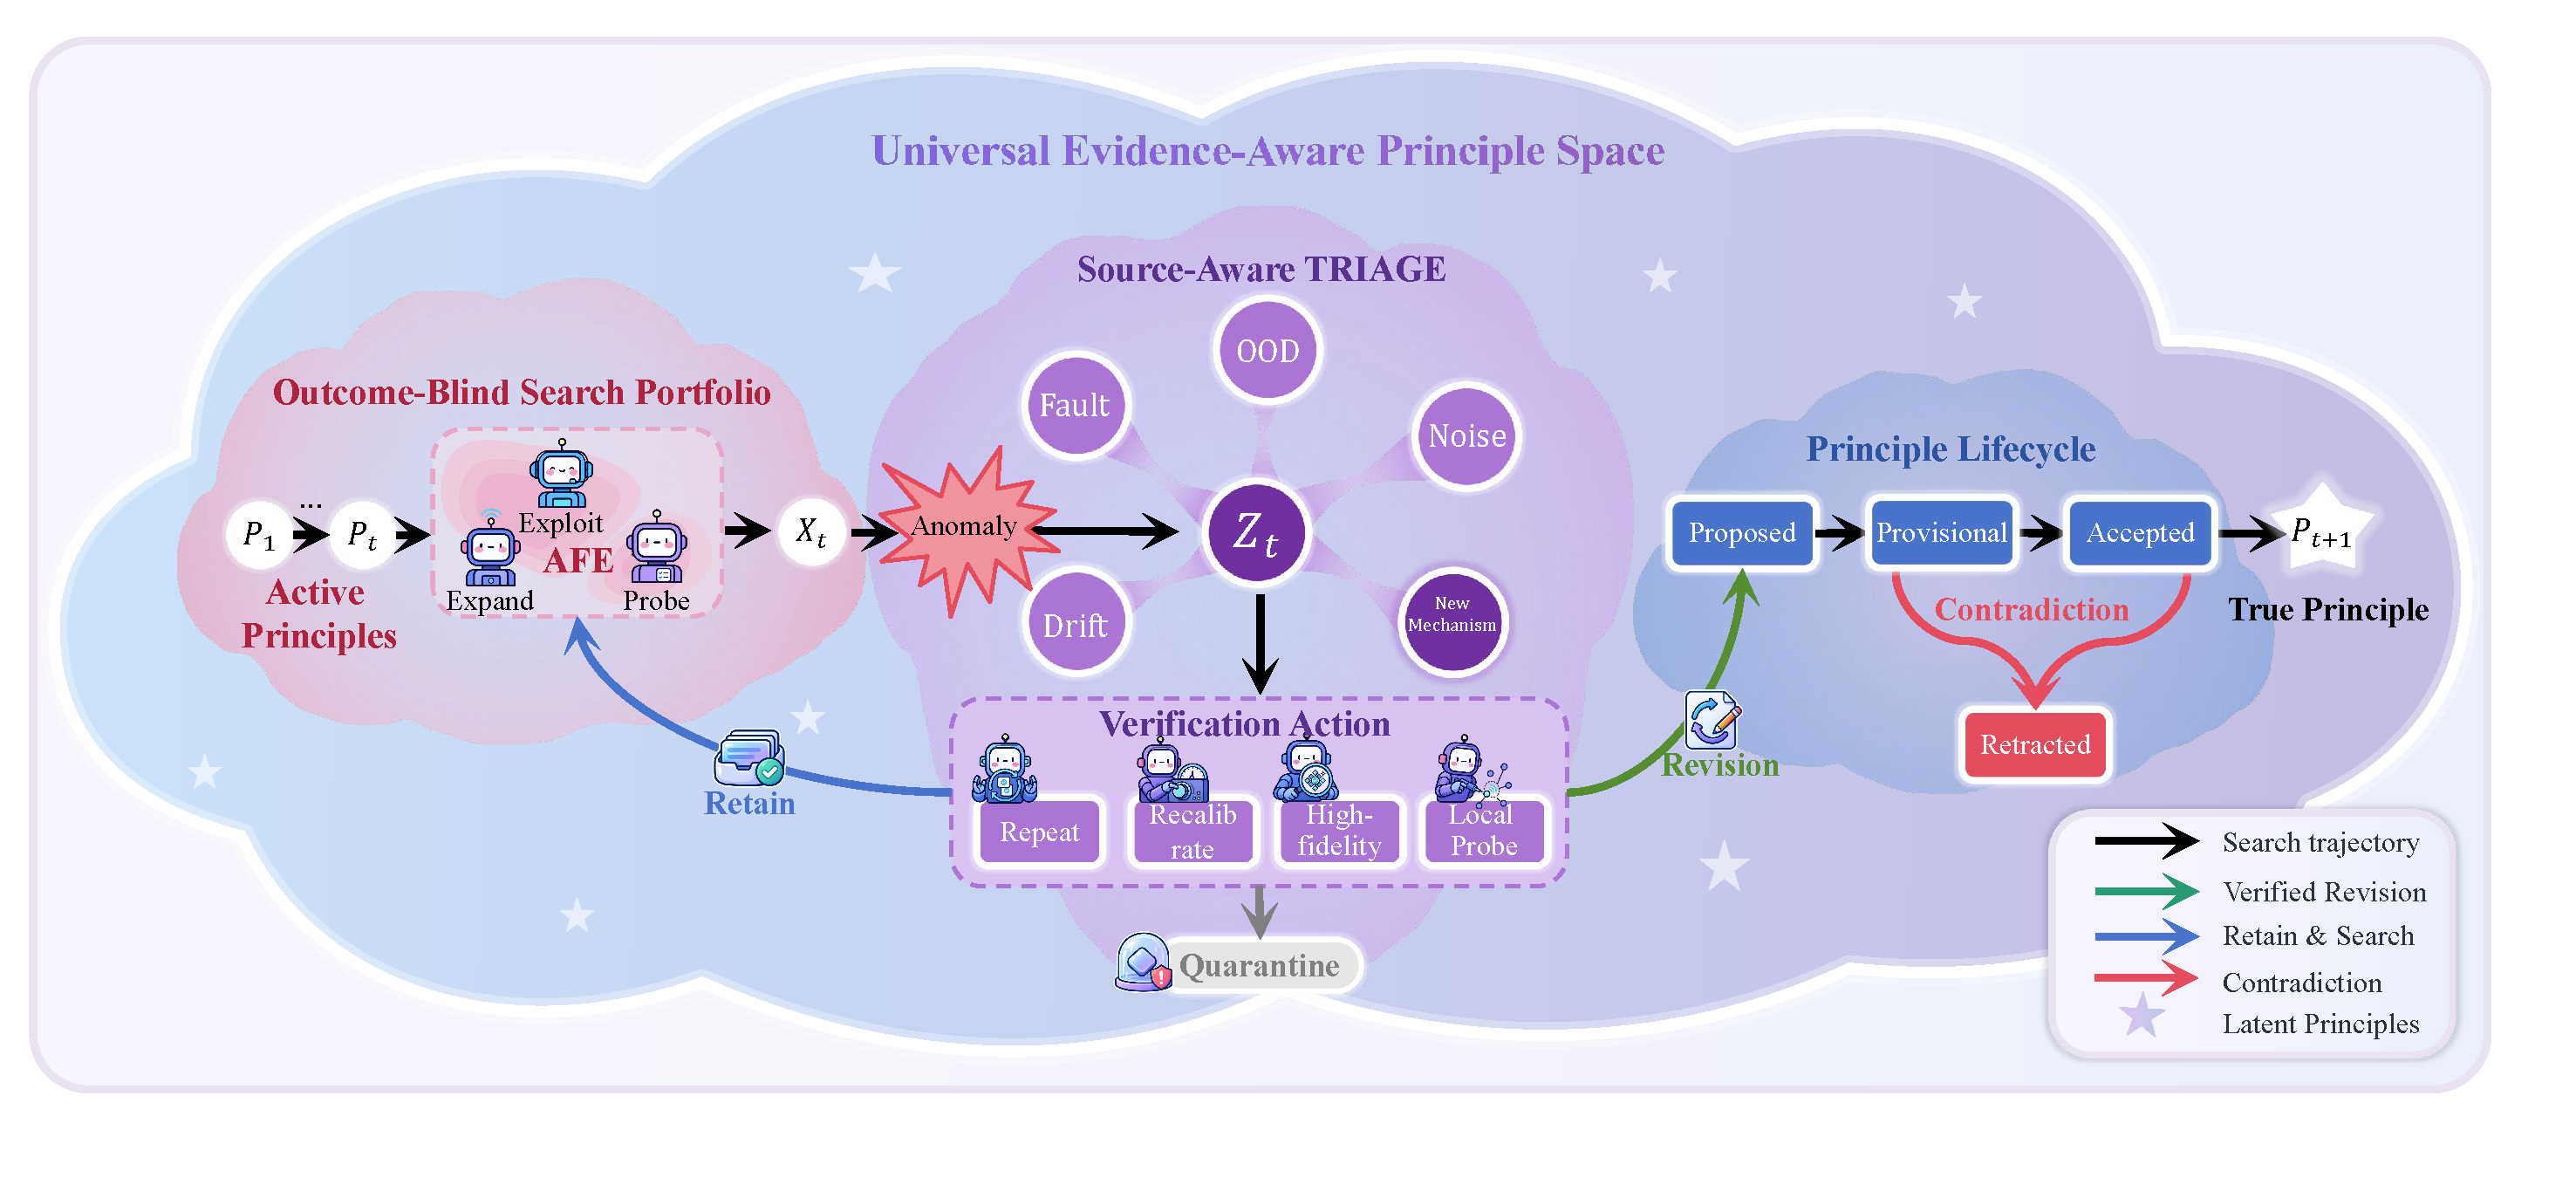
\includegraphics[width=\textwidth]{figures/fig_method_overview.pdf}
    \vspace{-0.6cm}
    \caption{\textbf{Overview of \method{}.} \textit{Left:} an outcome-blind AFE portfolio cycles candidate proposals $X_t$ across exploitation, frontier expansion, and mechanism-discriminating probes. \textit{Middle:} \triage{} attributes each anomalous residual to a latent source $Z_t$ and routes the observation to quarantine, search history, or principle revision. \textit{Right:} principles advance \textsc{Proposed} $\to$ \textsc{Provisional} $\to$ \textsc{Accepted} only with independent held-out support; contradictory evidence retracts them.}
    \label{fig:method-overview}
\end{figure*}

\section{Methodology}
\label{sec:methodology}

\subsection{Overview}

\triage{} changes one interface in a principle-evolving agent: the path from an anomalous observation to a persistent principle update. A high-surprisal outcome opens a diagnostic state, in which the controller may repeat the evaluation, consult another channel, or request a held-out probe; only reconciled evidence can affect principle status.

Two linked histories support this. A primary record stores the candidate, prediction, outcome, source channel, and metadata. A verification record stores a repeated, cross-channel, or held-out outcome with its cost and a pointer to the primary observation. Separating them keeps a verification result from silently re-entering search as a new observation, and makes the provenance of each principle update explicit. We write \triage{} for this admission protocol and \method{} for the integrated system of §\ref{sec:experiments}, which adds an outcome-blind Active Flow Expansion (AFE) portfolio. AFE decides where to search; \triage{} decides what may change a principle, so search stays exploratory without granting every promising observation the same epistemic standing (Figure~\ref{fig:method-overview}).

\subsection{Revision under Source Ambiguity}

At step $t$, the agent evaluates a candidate $x_t$ under principle state $\mathcal{P}_t$, obtaining outcome $y_t$ with metadata $m_t$ available before verification (batch identity, execution status, surrogate uncertainty); $h_t$ is the history of primary observations and actions, and the anomaly score $s_t$ summarizes the gap between $y_t$ and the prediction implied by $\mathcal{P}_t$.

We represent the ambiguity behind this discrepancy with a latent source variable:
\begin{equation}
\begin{split}
  Z_t \in \mathcal{Z} = \{ &\text{noise},\ \text{device fault},\ \text{execution failure},\ \text{surrogate mismatch},\\
  &\text{OOD input},\ \text{drift},\ \text{new mechanism}\}.
\end{split}
  \label{eq:sources}
\end{equation}
The true source is unobserved, and the same anomaly score can arise from several elements of $\mathcal{Z}$. A decision-theoretic account of this ambiguity starts from a posterior over sources,
\begin{equation}
 q_t(z) = p(z \mid h_t,y_t,m_t,\mathcal{P}_t) \propto p(y_t \mid x_t,z,m_t,\mathcal{P}_t) p(z \mid h_t,m_t,\mathcal{P}_t).
 \label{eq:posterior}
\end{equation}
Let $a_t\in\mathcal{A}=\{\text{repeat},\text{recalibrate},\text{high-fidelity},\text{local probe}\}$ denote verification actions with cost $C(a)$. Deciding between revision and retention involves asymmetric errors:
\begin{equation}
 L(d,z)=\ell_{\mathrm{FR}}\mathbb{1}[d=\revise,z\neq z_{\mathrm{mech}}] + \ell_{\mathrm{FM}}\mathbb{1}[d=\retain,z=z_{\mathrm{mech}}],
 \label{eq:loss}
\end{equation}
where $\ell_{\mathrm{FR}} \gg \ell_{\mathrm{FM}}$ penalizes corrupting persistent scientific principles much more heavily than missing a transient mechanism. The corresponding Bayes risk is $\mathcal{R}_t=\min_d\mathbb{E}_{q_t}[L(d,Z_t)]$, yielding the value-of-verification:
\begin{equation}
 V_t(a) = \mathcal{R}_t - \mathbb{E}_{v\sim p(v\mid\mathcal{D}_t,a)}[\mathcal{R}_{t+1}(a,v)] - \lambda_c C(a) - \lambda_f Q_{t+1}^{\mathrm{FR}}(a).
 \label{eq:utility}
\end{equation}
\paragraph{From Reference Model to Runtime Protocol.}
Equations~(\ref{eq:sources})--(\ref{eq:utility}) state what a correct revision decision requires; they are not executed at runtime. Estimating $q_t(z)$ needs a per-source likelihood $p(y_t\mid x_t,z,m_t,\mathcal{P}_t)$ that these settings do not provide: the evaluator is a black box and source labels are never observed. The design question is thus not how to recover $Z_t$, but how to decide correctly without recovering it. We take three properties from the reference model and realize each with an observable quantity:
\begin{enumerate}[nosep, leftmargin=12pt]
  \item \textbf{Ambiguity triggers verification, not revision.} Where the reference model acts on posterior mass spread across $\mathcal{Z}$, the runtime opens a diagnostic state whenever $s_t > \tau_{\mathrm{anom}} = 0.85$. Verification stays conditional, so cost is paid only on anomalies ($2.8$ extra calls per run)---the role of $\lambda_c C(a)$ in Equation~(\ref{eq:utility}).
  \item \textbf{Verification actions are ordered by discriminative power.} Instead of maximizing $V_t(a)$ online, actions escalate along a fixed order---same-channel repeat, cross-channel check, held-out probe---stopping once the evidence is decisive. That order is the standing ranking of $V_t(a)$ under Equation~(\ref{eq:loss}): repeats separate transient noise from persistent effects, cross-channel checks separate channel faults from signal, and only held-out probes separate an artifact from a mechanism.
  \item \textbf{The gate is asymmetric because the losses are.} With $\ell_{\mathrm{FR}} \gg \ell_{\mathrm{FM}}$, the two paths carry different burdens of proof. Same-channel agreement ($|y_t - v_t| \le \epsilon_{\mathrm{rep}} = 0.12$) admits an observation to search but never authorizes revision; revision also needs agreement with a distinct channel $c' = \arg\max_{c'' \neq c} p_{c''}^{\mathrm{trust}}$ ($|v_t^c - v_t^{c'}| \le \epsilon_{\mathrm{ind}} = 0.12$) and $k$ independent held-out records.
\end{enumerate}
The controller tracks per-channel reliability with a Beta posterior $r_c \sim \operatorname{Beta}(\alpha_c,\beta_c)$, $p_c^{\mathrm{trust}} = \alpha_c/(\alpha_c+\beta_c)$, incrementing $\alpha_c$ on agreement and $\beta_c$ on disagreement. Trust governs which channels are eligible to verify and flags degraded ones, but it never relaxes the standard of proof: $k$, $\tau_{\mathrm{gen}}$, and the tolerances are fixed a priori, so no channel earns the right to bypass held-out corroboration however reliable its history.

\subsection{Outcome-Blind Search Portfolio}

\method{} broadens candidate proposals across three structured roles: best-region exploitation, frontier expansion, and mechanism-discriminating probes~\citep{desanti2026actflow}. 

\begin{wrapfigure}[18]{r}{0.45\textwidth}
    \vspace{-12pt}
    \centering
    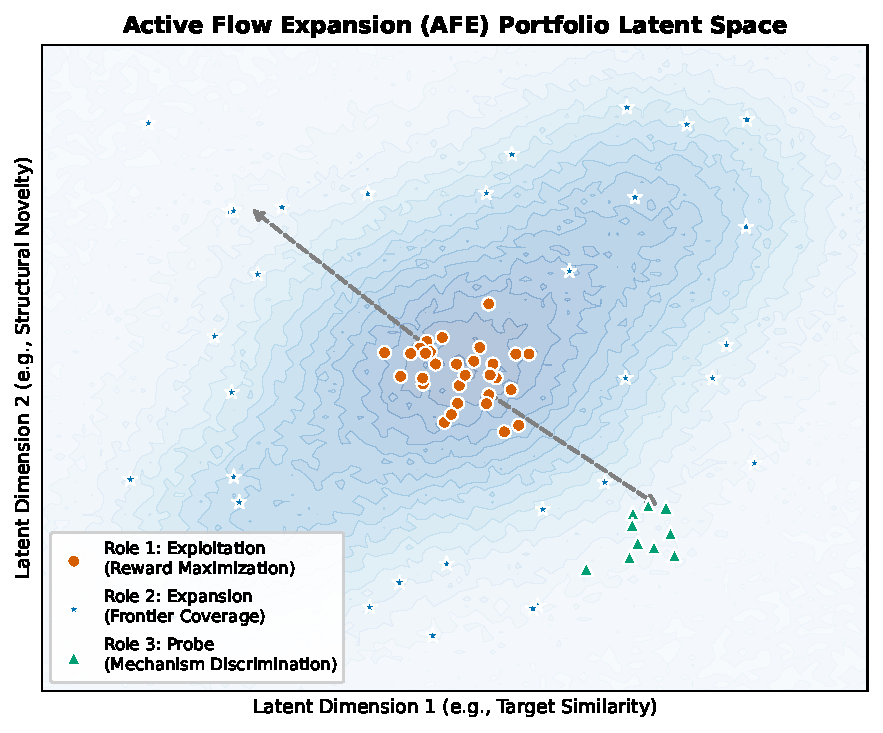
\includegraphics[width=\linewidth]{figures/fig_afe_manifold.pdf}
    \vspace{-6pt}
    \caption{\textbf{AFE portfolio (schematic).} Complementary candidate roles.}
    \label{fig:afe-manifold}
    \vspace{-6pt}
\end{wrapfigure}

\paragraph{Outcome-Blind Specification.}
``Outcome-blind'' means the proposal policy is \emph{gate-blind} and \emph{verifier-blind}: generators cycle deterministically through the roles with no access to verifier channels, latent sources $Z_t$, or gate states, so a quarantine or retraction cannot steer the next proposal. Surrogate reward $\hat{\mu}(x)$ and uncertainty $\hat{\sigma}(x)$ are refit each round from admitted primary observations only---quarantined records are excluded until reconciled---so a corrupted outcome cannot influence scoring through the surrogate either. For role $r$,
\begin{equation}
 A_r(x)=w_r^{\mu}\hat{\mu}(x)+w_r^{\sigma}\hat{\sigma}(x) + w_r^{n}N(x)+w_r^{d}D(x),
 \label{eq:afe}
\end{equation}
where $N(x)$ is distance from evaluated inputs and $D(x)$ descriptor novelty; role weights are fixed a priori (Appendix~\ref{app:hyperparams}) and Figure~\ref{fig:afe-manifold} shows the resulting geometry. \triage{} acts only after evaluation: agreement admits an observation to search, disagreement substitutes the verified median.

\subsection{Coherent Augmentation for Principles}

Each candidate principle stores a parent pointer, supporting/contradicting records, and a lifecycle state: $\textsc{Proposed} \to \textsc{Provisional} \to \textsc{Accepted}$ (or $\textsc{Retracted}$). The first supporting record makes a proposal provisional. A provisional principle is accepted if and only if
\begin{equation}
 P:\mathrm{provisional}\rightarrow\mathrm{accepted}
 \quad\Longleftrightarrow\quad
 \left|\{e\in E(P):e.\mathrm{ind}\wedge e.\mathrm{heldout}\wedge \mathrm{support}(e,P)\}\right|\geq k,
 \label{eq:gate}
\end{equation}
with $k=2$. Writing $\Delta_{\mathrm{heldout}}(e;P)$ for the held-out gain of $P$ measured by $e$, the three predicates are: $e.\mathrm{ind}$, the record comes from an evaluator process sharing no memory, cache, or random seed with the primary evaluator---a declared channel identity checked before the record counts, asserted at the process level rather than tested statistically; $e.\mathrm{heldout}$, the record is evaluated on a partition $X_{\mathrm{heldout}}$ with $X_{\mathrm{heldout}} \cap X_{\mathrm{train}} = \emptyset$, fixed before the run and hidden from the generator; and stance, $\mathrm{support}(e,P) = \mathbb{1}[\Delta_{\mathrm{heldout}}(e;P) \ge \tau_{\mathrm{gen}}]$ and $\mathrm{contradict}(e,P) = \mathbb{1}[\Delta_{\mathrm{heldout}}(e;P) \le -\tau_{\mathrm{gen}}]$ with $\tau_{\mathrm{gen}}=0.16$, leaving records inside the band uninformative. The symmetric margin is what separates an artifact from a mechanism: an artifact reproduces under repetition yet gives $\Delta_{\mathrm{heldout}} < \tau_{\mathrm{gen}}$, so it never reaches the count in Equation~(\ref{eq:gate}). Any record with $\mathrm{contradict}(e,P)=1$ retracts $P$ and, recursively, every principle listing $P$ as a parent. Pseudocode is in Appendix~\ref{app:pseudocode}.

\section{Experiments}
\label{sec:experiments}

We evaluate \method{} across three complementary dimensions: (1) downstream optimization performance across four scientific discovery tasks under three backbone LLMs; (2) component ablations isolating search expansion from evidence admission; and (3) controlled stress tests targeting evaluator corruption, hidden anomaly sources, mechanism reversal, proxy exploitation, and cross-harness deployment.

\subsection{Experiment Setup}
\label{sec:matched}

\paragraph{Tasks and Baselines.} We use four discovery environments from \pievo{}~\citep{pu2026pievo}: Molecular Bio-activity Optimization (MBO), Nanomaterial Optical Property Optimization (NHO), Superconductor Optimization (SPO), and Transition Metal Complex Optimization (TMC), against seven baselines: Vanilla MAS, ReAct~\citep{yao2023reactsynergizingreasoningacting}, AI Scientist v1~\citep{lu2024aiscientist}, AI Scientist v2~\citep{yamada2025aiscientistv2workshoplevelautomated}, AI Researcher~\citep{tang2025airesearcherautonomousscientificinnovation}, PiFlow~\citep{pu2026piflowprincipleawarescientificdiscovery}, and \pievo{}~\citep{pu2026pievo}.

\paragraph{Implementation Details.} We evaluate three backbones---Qwen3-235B, Gemini-2.5-Flash-Lite, GPT-5.6-Luna---in direct execution mode without extended chain-of-thought, over three fixed seeds (0, 1, 2) at a budget of 24 primary evaluations: 96 runs per model, 288 trajectories. Gate parameters are fixed a priori across all tasks and backbones: $\tau_{\mathrm{anom}}=0.85$, $\epsilon_{\mathrm{rep}}=\epsilon_{\mathrm{ind}}=0.12$, $\tau_{\mathrm{gen}}=0.16$, $k=2$ (full specification and sensitivity sweeps in Appendix~\ref{app:hyperparams}). 

\paragraph{Evaluation Metrics.} With $y_{1:T}$ the primary outcomes of a run: (1)~\textbf{Solution Quality} (SQ, \%, $\uparrow$) is $100\cdot\max_t y_t/\mu_{\mathrm{ref}}$; (2)~\textbf{AUOC} (\%, $\uparrow$) is $100\cdot\frac{1}{T}\sum_{t}\max_{t'\leq t} y_{t'}/\mu_{\mathrm{ref}}$, crediting how early quality is reached; (3)~\textbf{APD} ($\uparrow$) is mean pairwise cosine distance between proposed candidates under Qwen3-Embedding-0.6B. References are $\mu_{\mathrm{ref}}=6.5$ (MBO), $2.0$ (NHO), $298.5$ (SPO), $493.8$ (TMC), from \pievo{}~\citep{pu2026pievo}. These are published reference values, not attainable upper bounds, so SQ passes $100$ when a run beats the reference; we apply no clipping.

\begin{table*}[!ht]
\caption{Solution Quality (SQ, \%) across four discovery tasks and three backbone LLMs. Entries report mean $\pm$ SD over three seeds; averages are computed across tasks. Bold indicates the best result within each backbone.}
\label{tab:main-sq}
\centering
\small
\resizebox{\linewidth}{!}{%
\begin{tabular}{l | cccc | c}
\toprule
\textbf{Model / Method} & \textbf{MBO} & \textbf{NHO} & \textbf{SPO} & \textbf{TMC} & \textbf{Average} \\
\midrule
\multicolumn{6}{l}{\textbf{Qwen3-235B (No Thinking)}} \\
\midrule
Vanilla MAS & 83.35 \textcolor{gray}{\scriptsize $\pm$ 29.95} & 52.83 \textcolor{gray}{\scriptsize $\pm$ 20.36} & 37.29 \textcolor{gray}{\scriptsize $\pm$ 0.75} & 56.34 \textcolor{gray}{\scriptsize $\pm$ 3.69} & 57.45  \\
ReAct & 75.48 \textcolor{gray}{\scriptsize $\pm$ 4.94} \textcolor{red}{\scriptsize $\downarrow$ 0.9x} & 61.95 \textcolor{gray}{\scriptsize $\pm$ 17.08} \textcolor{purple}{\scriptsize $\uparrow$ 1.2x} & 37.49 \textcolor{gray}{\scriptsize $\pm$ 0.46} & 72.80 \textcolor{gray}{\scriptsize $\pm$ 4.48} \textcolor{purple}{\scriptsize $\uparrow$ 1.3x} & 61.93  \textcolor{purple}{\scriptsize $\uparrow$ 1.1x} \\
AI Scientist v1 & 73.37 \textcolor{gray}{\scriptsize $\pm$ 39.82} \textcolor{red}{\scriptsize $\downarrow$ 0.9x} & 41.50 \textcolor{gray}{\scriptsize $\pm$ 3.12} \textcolor{red}{\scriptsize $\downarrow$ 0.8x} & 37.04 \textcolor{gray}{\scriptsize $\pm$ 0.61} & 63.96 \textcolor{gray}{\scriptsize $\pm$ 8.93} \textcolor{purple}{\scriptsize $\uparrow$ 1.1x} & 53.97  \textcolor{red}{\scriptsize $\downarrow$ 0.9x} \\
AI Scientist v2 & 84.40 \textcolor{gray}{\scriptsize $\pm$ 20.07} & 52.34 \textcolor{gray}{\scriptsize $\pm$ 15.56} & 41.40 \textcolor{gray}{\scriptsize $\pm$ 1.15} \textcolor{purple}{\scriptsize $\uparrow$ 1.1x} & 63.52 \textcolor{gray}{\scriptsize $\pm$ 2.86} \textcolor{purple}{\scriptsize $\uparrow$ 1.1x} & 60.42  \textcolor{purple}{\scriptsize $\uparrow$ 1.1x} \\
AI Researcher & 105.70 \textcolor{gray}{\scriptsize $\pm$ 21.92} \textcolor{purple}{\scriptsize $\uparrow$ 1.3x} & 37.21 \textcolor{gray}{\scriptsize $\pm$ 5.68} \textcolor{red}{\scriptsize $\downarrow$ 0.7x} & 37.39 \textcolor{gray}{\scriptsize $\pm$ 0.85} & 78.80 \textcolor{gray}{\scriptsize $\pm$ 3.76} \textcolor{purple}{\scriptsize $\uparrow$ 1.4x} & 64.78  \textcolor{purple}{\scriptsize $\uparrow$ 1.1x} \\
PiFlow & 81.89 \textcolor{gray}{\scriptsize $\pm$ 30.49} & 56.15 \textcolor{gray}{\scriptsize $\pm$ 15.23} \textcolor{purple}{\scriptsize $\uparrow$ 1.1x} & 37.21 \textcolor{gray}{\scriptsize $\pm$ 0.52} & 54.58 \textcolor{gray}{\scriptsize $\pm$ 2.70} & 57.46  \\
\pievo{} & 97.84 \textcolor{gray}{\scriptsize $\pm$ 27.49} \textcolor{purple}{\scriptsize $\uparrow$ 1.2x} & 65.53 \textcolor{gray}{\scriptsize $\pm$ 21.90} \textcolor{purple}{\scriptsize $\uparrow$ 1.2x} & 37.71 \textcolor{gray}{\scriptsize $\pm$ 0.53} & 80.30 \textcolor{gray}{\scriptsize $\pm$ 4.57} \textcolor{purple}{\scriptsize $\uparrow$ 1.4x} & 70.35  \textcolor{purple}{\scriptsize $\uparrow$ 1.2x} \\
\textbf{Triage-PiEvo (ours)} & \textbf{132.00} \textcolor{gray}{\scriptsize $\pm$ 9.84} \textcolor{purple}{\scriptsize $\uparrow$ 1.6x} & \textbf{72.89} \textcolor{gray}{\scriptsize $\pm$ 17.80} \textcolor{purple}{\scriptsize $\uparrow$ 1.4x} & \textbf{42.00} \textcolor{gray}{\scriptsize $\pm$ 1.20} \textcolor{purple}{\scriptsize $\uparrow$ 1.1x} & \textbf{81.50} \textcolor{gray}{\scriptsize $\pm$ 4.02} \textcolor{purple}{\scriptsize $\uparrow$ 1.4x} & \textbf{82.10}  \textcolor{purple}{\scriptsize $\uparrow$ 1.4x} \\
\midrule
\multicolumn{6}{l}{\textbf{Gemini-2.5-Flash-Lite (No Thinking)}} \\
\midrule
Vanilla MAS & 62.06 \textcolor{gray}{\scriptsize $\pm$ 14.09} & 71.98 \textcolor{gray}{\scriptsize $\pm$ 1.01} & 36.95 \textcolor{gray}{\scriptsize $\pm$ 0.46} & 66.64 \textcolor{gray}{\scriptsize $\pm$ 17.42} & 59.41  \\
ReAct & 58.83 \textcolor{gray}{\scriptsize $\pm$ 6.44} \textcolor{red}{\scriptsize $\downarrow$ 0.9x} & 69.90 \textcolor{gray}{\scriptsize $\pm$ 1.50} & 32.06 \textcolor{gray}{\scriptsize $\pm$ 5.75} \textcolor{red}{\scriptsize $\downarrow$ 0.9x} & 56.31 \textcolor{gray}{\scriptsize $\pm$ 2.37} \textcolor{red}{\scriptsize $\downarrow$ 0.8x} & 54.27  \textcolor{red}{\scriptsize $\downarrow$ 0.9x} \\
AI Scientist v1 & 75.60 \textcolor{gray}{\scriptsize $\pm$ 22.03} \textcolor{purple}{\scriptsize $\uparrow$ 1.2x} & 73.58 \textcolor{gray}{\scriptsize $\pm$ 2.23} & 37.86 \textcolor{gray}{\scriptsize $\pm$ 2.55} & 55.70 \textcolor{gray}{\scriptsize $\pm$ 2.62} \textcolor{red}{\scriptsize $\downarrow$ 0.8x} & 60.68  \\
AI Scientist v2 & 99.30 \textcolor{gray}{\scriptsize $\pm$ 22.73} \textcolor{purple}{\scriptsize $\uparrow$ 1.6x} & 74.87 \textcolor{gray}{\scriptsize $\pm$ 2.00} & 30.74 \textcolor{gray}{\scriptsize $\pm$ 3.96} \textcolor{red}{\scriptsize $\downarrow$ 0.8x} & 54.80 \textcolor{gray}{\scriptsize $\pm$ 4.09} \textcolor{red}{\scriptsize $\downarrow$ 0.8x} & 64.93  \textcolor{purple}{\scriptsize $\uparrow$ 1.1x} \\
AI Researcher & 66.47 \textcolor{gray}{\scriptsize $\pm$ 16.70} \textcolor{purple}{\scriptsize $\uparrow$ 1.1x} & 65.39 \textcolor{gray}{\scriptsize $\pm$ 9.16} \textcolor{red}{\scriptsize $\downarrow$ 0.9x} & 31.62 \textcolor{gray}{\scriptsize $\pm$ 3.82} \textcolor{red}{\scriptsize $\downarrow$ 0.9x} & 63.46 \textcolor{gray}{\scriptsize $\pm$ 13.85} & 56.74  \\
PiFlow & 96.59 \textcolor{gray}{\scriptsize $\pm$ 11.71} \textcolor{purple}{\scriptsize $\uparrow$ 1.6x} & 74.24 \textcolor{gray}{\scriptsize $\pm$ 4.06} & 34.91 \textcolor{gray}{\scriptsize $\pm$ 3.66} \textcolor{red}{\scriptsize $\downarrow$ 0.9x} & 68.22 \textcolor{gray}{\scriptsize $\pm$ 8.71} & 68.49  \textcolor{purple}{\scriptsize $\uparrow$ 1.2x} \\
\pievo{} & 72.59 \textcolor{gray}{\scriptsize $\pm$ 6.70} \textcolor{purple}{\scriptsize $\uparrow$ 1.2x} & 81.00 \textcolor{gray}{\scriptsize $\pm$ 3.06} \textcolor{purple}{\scriptsize $\uparrow$ 1.1x} & 38.02 \textcolor{gray}{\scriptsize $\pm$ 0.50} & 78.50 \textcolor{gray}{\scriptsize $\pm$ 7.60} \textcolor{purple}{\scriptsize $\uparrow$ 1.2x} & 67.53  \textcolor{purple}{\scriptsize $\uparrow$ 1.1x} \\
\textbf{Triage-PiEvo (ours)} & \textbf{115.00} \textcolor{gray}{\scriptsize $\pm$ 10.00} \textcolor{purple}{\scriptsize $\uparrow$ 1.9x} & \textbf{83.00} \textcolor{gray}{\scriptsize $\pm$ 5.00} \textcolor{purple}{\scriptsize $\uparrow$ 1.2x} & \textbf{40.50} \textcolor{gray}{\scriptsize $\pm$ 4.00} \textcolor{purple}{\scriptsize $\uparrow$ 1.1x} & \textbf{80.00} \textcolor{gray}{\scriptsize $\pm$ 4.00} \textcolor{purple}{\scriptsize $\uparrow$ 1.2x} & \textbf{79.63}  \textcolor{purple}{\scriptsize $\uparrow$ 1.3x} \\
\midrule
\multicolumn{6}{l}{\textbf{GPT-5.6-Luna (No Thinking)}} \\
\midrule
Vanilla MAS & 91.84 \textcolor{gray}{\scriptsize $\pm$ 18.08} & 66.26 \textcolor{gray}{\scriptsize $\pm$ 7.14} & 36.42 \textcolor{gray}{\scriptsize $\pm$ 0.50} & 68.07 \textcolor{gray}{\scriptsize $\pm$ 3.91} & 65.65  \\
ReAct & 132.00 \textcolor{gray}{\scriptsize $\pm$ 22.98} \textcolor{purple}{\scriptsize $\uparrow$ 1.4x} & 69.98 \textcolor{gray}{\scriptsize $\pm$ 0.14} \textcolor{purple}{\scriptsize $\uparrow$ 1.1x} & 36.22 \textcolor{gray}{\scriptsize $\pm$ 0.34} & 65.37 \textcolor{gray}{\scriptsize $\pm$ 5.39} & 75.89  \textcolor{purple}{\scriptsize $\uparrow$ 1.2x} \\
AI Scientist v1 & 91.16 \textcolor{gray}{\scriptsize $\pm$ 19.35} & 53.02 \textcolor{gray}{\scriptsize $\pm$ 12.32} \textcolor{red}{\scriptsize $\downarrow$ 0.8x} & 35.52 \textcolor{gray}{\scriptsize $\pm$ 4.90} & 62.44 \textcolor{gray}{\scriptsize $\pm$ 6.24} \textcolor{red}{\scriptsize $\downarrow$ 0.9x} & 60.54  \textcolor{red}{\scriptsize $\downarrow$ 0.9x} \\
AI Scientist v2 & 89.63 \textcolor{gray}{\scriptsize $\pm$ 31.45} & 65.13 \textcolor{gray}{\scriptsize $\pm$ 15.46} & 36.77 \textcolor{gray}{\scriptsize $\pm$ 5.05} & 58.29 \textcolor{gray}{\scriptsize $\pm$ 0.95} \textcolor{red}{\scriptsize $\downarrow$ 0.9x} & 62.46  \\
AI Researcher & 77.86 \textcolor{gray}{\scriptsize $\pm$ 15.38} \textcolor{red}{\scriptsize $\downarrow$ 0.8x} & 73.92 \textcolor{gray}{\scriptsize $\pm$ 9.01} \textcolor{purple}{\scriptsize $\uparrow$ 1.1x} & 36.28 \textcolor{gray}{\scriptsize $\pm$ 0.24} & 72.93 \textcolor{gray}{\scriptsize $\pm$ 2.06} \textcolor{purple}{\scriptsize $\uparrow$ 1.1x} & 65.25  \\
PiFlow & 128.77 \textcolor{gray}{\scriptsize $\pm$ 18.74} \textcolor{purple}{\scriptsize $\uparrow$ 1.4x} & 46.62 \textcolor{gray}{\scriptsize $\pm$ 17.77} \textcolor{red}{\scriptsize $\downarrow$ 0.7x} & 31.49 \textcolor{gray}{\scriptsize $\pm$ 5.94} \textcolor{red}{\scriptsize $\downarrow$ 0.9x} & 59.59 \textcolor{gray}{\scriptsize $\pm$ 5.23} \textcolor{red}{\scriptsize $\downarrow$ 0.9x} & 66.62  \\
\pievo{} & 69.75 \textcolor{gray}{\scriptsize $\pm$ 6.20} \textcolor{red}{\scriptsize $\downarrow$ 0.8x} & 67.82 \textcolor{gray}{\scriptsize $\pm$ 10.87} & 37.41 \textcolor{gray}{\scriptsize $\pm$ 0.53} & 76.50 \textcolor{gray}{\scriptsize $\pm$ 1.78} \textcolor{purple}{\scriptsize $\uparrow$ 1.1x} & 62.87  \\
\textbf{Triage-PiEvo (ours)} & \textbf{136.00} \textcolor{gray}{\scriptsize $\pm$ 9.84} \textcolor{purple}{\scriptsize $\uparrow$ 1.5x} & \textbf{78.18} \textcolor{gray}{\scriptsize $\pm$ 5.44} \textcolor{purple}{\scriptsize $\uparrow$ 1.2x} & \textbf{40.80} \textcolor{gray}{\scriptsize $\pm$ 5.70} \textcolor{purple}{\scriptsize $\uparrow$ 1.1x} & \textbf{78.50} \textcolor{gray}{\scriptsize $\pm$ 3.75} \textcolor{purple}{\scriptsize $\uparrow$ 1.2x} & \textbf{83.37}  \textcolor{purple}{\scriptsize $\uparrow$ 1.3x} \\
\bottomrule
\end{tabular}%
}
\end{table*}

\subsection{Matched Downstream Performance}
\label{sec:performance}

Table~\ref{tab:main-sq} reports terminal Solution Quality. \method{} reaches the highest average SQ for each backbone---$82.10$, $79.63$, and $83.37$---improving on the strongest baseline for that backbone by $11.75$, $11.14$, and $7.48$ points. That strongest baseline differs across backbones (\pievo{}, PiFlow, ReAct), and none leads on more than one: a method tuned to one backbone's failure profile does not carry to another, whereas \method{} is first on all three.

The per-task breakdown locates the gain. It concentrates on MBO ($132.00$, $115.00$, $136.00$), the task with the widest baseline spread---on Qwen3-235B, from $73.37$ to $105.70$---and therefore the most room for a principle to be either genuinely revised or corrupted by a spurious outcome. SPO is the opposite: every method lands between $30.74$ and $42.00$ and our margin narrows to $0.6$--$3.4$ points. Gains track how much of a task's difficulty lies in deciding what to believe rather than where to search, which is what an evidence-admission layer should predict. Variance moves the same way: on Qwen3-235B MBO, \method{} reports $\pm 9.84$ against $\pm 27.49$ for the closest baseline and $\pm 39.82$ for the widest, and on all three backbones our MBO spread stays below the baseline median. Since the gate keeps unreconciled outcomes out of persistent state, suppressing seed-to-seed spread is a more direct signature of it working than the mean shift is.

This table evaluates the integrated system and does not attribute the gain to either component; §\ref{sec:ablation} separates them. AUOC and APD appear in Table~\ref{tab:main-apd-auoc}, where higher peak SQ coincides with broader coverage and faster optimization---the gate does not buy reliability by narrowing exploration. Figure~\ref{fig:qwen-convergence} shows best-so-far trajectories with Qwen3-235B: \method{} opens a margin within 5 iterations and holds it to the terminal rounds, at $+13.6\%$ runtime (Appendix~\ref{app:runtime}).

\begin{figure*}[t]
    \centering
    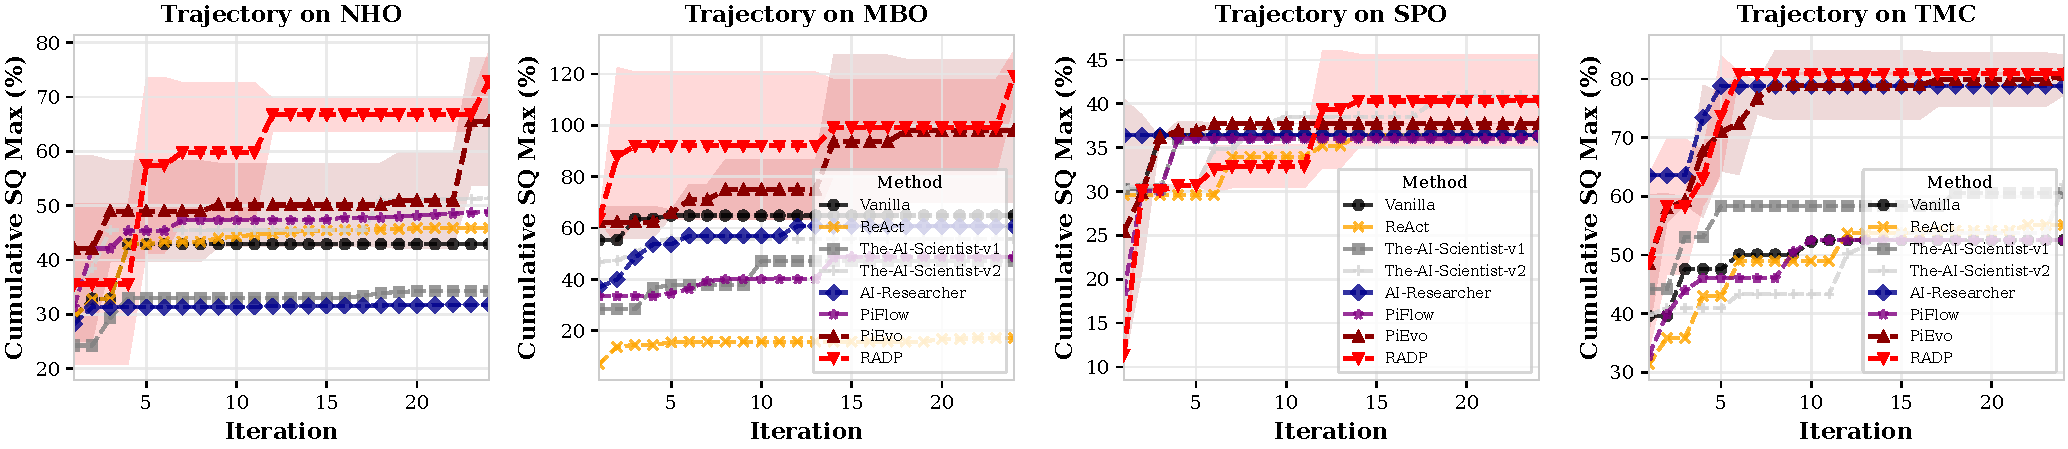
\includegraphics[width=\textwidth]{figures/fig_qwen_convergence.pdf}
    \vspace{-0.65cm}
    \caption{\textbf{Best-so-far optimization trajectories over 24 primary evaluations across four benchmark discovery tasks with Qwen3-235B.} Curves report the empirical mean over three independent seeds; shaded ribbons indicate $\pm 1$ standard deviation. Across all scientific domains, \method{} rapidly accumulates high-quality candidates and sustains the highest terminal solution quality.}
    \label{fig:qwen-convergence}
\end{figure*}

\begin{table*}[!ht]
\caption{Average Pairwise Distance (APD) and Area Under the Optimisation Curve (AUOC) across four tasks and three backbone LLMs. Entries report mean $\pm$ SD over three seeds. Higher APD indicates broader candidate coverage, while higher AUOC indicates faster accumulation of high-quality candidates.}
\label{tab:main-apd-auoc}
\centering
\small
\setlength{\tabcolsep}{2pt}
\resizebox{\linewidth}{!}{%
\begin{tabular}{l | cc | cc | cc | cc | cc}
\toprule
\textbf{Model / Method} & \multicolumn{2}{c}{\textbf{MBO}} & \multicolumn{2}{c}{\textbf{NHO}} & \multicolumn{2}{c}{\textbf{SPO}} & \multicolumn{2}{c}{\textbf{TMC}} & \multicolumn{2}{c}{\textbf{Average}} \\
 & \textbf{APD} $\uparrow$ & \textbf{AUOC} $\uparrow$ & \textbf{APD} $\uparrow$ & \textbf{AUOC} $\uparrow$ & \textbf{APD} $\uparrow$ & \textbf{AUOC} $\uparrow$ & \textbf{APD} $\uparrow$ & \textbf{AUOC} $\uparrow$ & \textbf{Avg APD} $\uparrow$ & \textbf{Avg AUOC} $\uparrow$ \\
\midrule
\multicolumn{11}{l}{\textbf{Qwen3-235B (No Thinking)}} \\
\midrule
Vanilla MAS & 53.58\textcolor{gray}{\tiny$\pm$15.25} & 70.09\textcolor{gray}{\tiny$\pm$17.75} & 32.23\textcolor{gray}{\tiny$\pm$3.72} & 49.33\textcolor{gray}{\tiny$\pm$17.82} & 52.03\textcolor{gray}{\tiny$\pm$1.05} & 36.34\textcolor{gray}{\tiny$\pm$0.38} & 51.89\textcolor{gray}{\tiny$\pm$3.85} & 52.67\textcolor{gray}{\tiny$\pm$3.49} & 47.43 & 52.11 \\
ReAct & 59.43\textcolor{gray}{\tiny$\pm$8.60} & 70.58\textcolor{gray}{\tiny$\pm$7.95} & \textbf{33.31}\textcolor{gray}{\tiny$\pm$1.86} & 47.46\textcolor{gray}{\tiny$\pm$7.04} & 56.13\textcolor{gray}{\tiny$\pm$4.49} & 35.74\textcolor{gray}{\tiny$\pm$0.76} & 72.93\textcolor{gray}{\tiny$\pm$0.33} & 66.95\textcolor{gray}{\tiny$\pm$4.67} & 55.45 \textcolor{purple}{\small $\uparrow$ 1.2x} & 55.18 \textcolor{purple}{\small $\uparrow$ 1.1x} \\
AI Scientist v1 & 52.93\textcolor{gray}{\tiny$\pm$15.22} & 56.16\textcolor{gray}{\tiny$\pm$26.05} & 32.98\textcolor{gray}{\tiny$\pm$2.32} & 38.84\textcolor{gray}{\tiny$\pm$2.06} & 42.55\textcolor{gray}{\tiny$\pm$5.61} & 35.62\textcolor{gray}{\tiny$\pm$1.46} & 64.43\textcolor{gray}{\tiny$\pm$7.02} & 57.50\textcolor{gray}{\tiny$\pm$6.15} & 48.22 & 47.03 \textcolor{red}{\small $\downarrow$ 0.9x} \\
AI Scientist v2 & 60.26\textcolor{gray}{\tiny$\pm$10.57} & 76.03\textcolor{gray}{\tiny$\pm$7.92} & 28.39\textcolor{gray}{\tiny$\pm$3.49} & 39.51\textcolor{gray}{\tiny$\pm$3.29} & 48.18\textcolor{gray}{\tiny$\pm$1.41} & 37.03\textcolor{gray}{\tiny$\pm$0.22} & 55.66\textcolor{gray}{\tiny$\pm$2.28} & 54.75\textcolor{gray}{\tiny$\pm$6.66} & 48.12 & 51.83 \\
AI Researcher & 59.17\textcolor{gray}{\tiny$\pm$3.77} & 89.21\textcolor{gray}{\tiny$\pm$19.08} & 25.51\textcolor{gray}{\tiny$\pm$3.45} & 34.51\textcolor{gray}{\tiny$\pm$3.80} & 47.62\textcolor{gray}{\tiny$\pm$3.55} & 36.82\textcolor{gray}{\tiny$\pm$0.41} & 52.46\textcolor{gray}{\tiny$\pm$6.03} & 74.19\textcolor{gray}{\tiny$\pm$0.70} & 46.19 & 58.68 \textcolor{purple}{\small $\uparrow$ 1.1x} \\
PiFlow & 64.99\textcolor{gray}{\tiny$\pm$2.39} & 64.04\textcolor{gray}{\tiny$\pm$14.87} & 28.07\textcolor{gray}{\tiny$\pm$1.85} & 52.93\textcolor{gray}{\tiny$\pm$15.82} & 51.24\textcolor{gray}{\tiny$\pm$4.14} & 35.90\textcolor{gray}{\tiny$\pm$1.33} & 57.76\textcolor{gray}{\tiny$\pm$3.35} & 50.26\textcolor{gray}{\tiny$\pm$1.85} & 50.52 \textcolor{purple}{\small $\uparrow$ 1.1x} & 50.78 \\
\pievo{} & 63.41\textcolor{gray}{\tiny$\pm$10.78} & 84.14\textcolor{gray}{\tiny$\pm$16.22} & 23.80\textcolor{gray}{\tiny$\pm$5.23} & 52.50\textcolor{gray}{\tiny$\pm$13.36} & 54.41\textcolor{gray}{\tiny$\pm$1.42} & 36.83\textcolor{gray}{\tiny$\pm$0.86} & 71.76\textcolor{gray}{\tiny$\pm$2.58} & 74.93\textcolor{gray}{\tiny$\pm$5.05} & 53.35 \textcolor{purple}{\small $\uparrow$ 1.1x} & 62.10 \textcolor{purple}{\small $\uparrow$ 1.2x} \\
\textbf{Triage-PiEvo (ours)} & \textbf{73.71}\textcolor{gray}{\tiny$\pm$2.86} & \textbf{110.00}\textcolor{gray}{\tiny$\pm$18.41} & 23.67\textcolor{gray}{\tiny$\pm$0.79} & \textbf{61.21}\textcolor{gray}{\tiny$\pm$11.52} & \textbf{57.34}\textcolor{gray}{\tiny$\pm$0.26} & \textbf{38.50}\textcolor{gray}{\tiny$\pm$1.80} & \textbf{74.20}\textcolor{gray}{\tiny$\pm$1.41} & \textbf{77.20}\textcolor{gray}{\tiny$\pm$2.95} & \textbf{57.23} \textcolor{purple}{\small $\uparrow$ 1.2x} & \textbf{71.73} \textcolor{purple}{\small $\uparrow$ 1.4x} \\
\midrule
\multicolumn{11}{l}{\textbf{Gemini-2.5-Flash-Lite (No Thinking)}} \\
\midrule
Vanilla MAS & 65.06\textcolor{gray}{\tiny$\pm$5.46} & 46.01\textcolor{gray}{\tiny$\pm$15.24} & 33.55\textcolor{gray}{\tiny$\pm$0.90} & 61.71\textcolor{gray}{\tiny$\pm$2.41} & 53.65\textcolor{gray}{\tiny$\pm$1.10} & 35.45\textcolor{gray}{\tiny$\pm$0.05} & 57.23\textcolor{gray}{\tiny$\pm$5.29} & 62.88\textcolor{gray}{\tiny$\pm$15.97} & 52.37 & 51.51 \\
ReAct & 62.08\textcolor{gray}{\tiny$\pm$1.15} & 44.54\textcolor{gray}{\tiny$\pm$2.54} & 34.46\textcolor{gray}{\tiny$\pm$0.57} & 58.08\textcolor{gray}{\tiny$\pm$5.33} & 42.17\textcolor{gray}{\tiny$\pm$12.13} & 25.95\textcolor{gray}{\tiny$\pm$8.19} & 52.75\textcolor{gray}{\tiny$\pm$5.72} & 52.03\textcolor{gray}{\tiny$\pm$0.12} & 47.87 \textcolor{red}{\small $\downarrow$ 0.9x} & 45.15 \textcolor{red}{\small $\downarrow$ 0.9x} \\
AI Scientist v1 & 52.02\textcolor{gray}{\tiny$\pm$15.45} & 58.73\textcolor{gray}{\tiny$\pm$5.53} & 33.13\textcolor{gray}{\tiny$\pm$0.89} & 64.99\textcolor{gray}{\tiny$\pm$5.57} & 47.13\textcolor{gray}{\tiny$\pm$4.98} & 33.96\textcolor{gray}{\tiny$\pm$1.93} & 56.53\textcolor{gray}{\tiny$\pm$1.71} & 51.60\textcolor{gray}{\tiny$\pm$0.09} & 47.20 \textcolor{red}{\small $\downarrow$ 0.9x} & 52.32 \\
AI Scientist v2 & 46.27\textcolor{gray}{\tiny$\pm$12.65} & 59.35\textcolor{gray}{\tiny$\pm$11.81} & \textbf{35.09}\textcolor{gray}{\tiny$\pm$0.38} & 67.18\textcolor{gray}{\tiny$\pm$1.82} & 43.28\textcolor{gray}{\tiny$\pm$0.12} & 24.33\textcolor{gray}{\tiny$\pm$7.17} & 42.16\textcolor{gray}{\tiny$\pm$9.83} & 52.77\textcolor{gray}{\tiny$\pm$3.83} & 41.70 \textcolor{red}{\small $\downarrow$ 0.8x} & 50.91 \\
AI Researcher & 60.38\textcolor{gray}{\tiny$\pm$7.64} & 45.98\textcolor{gray}{\tiny$\pm$15.08} & 33.16\textcolor{gray}{\tiny$\pm$3.51} & 58.94\textcolor{gray}{\tiny$\pm$6.79} & 41.65\textcolor{gray}{\tiny$\pm$9.04} & 28.78\textcolor{gray}{\tiny$\pm$2.15} & 55.97\textcolor{gray}{\tiny$\pm$2.51} & 59.77\textcolor{gray}{\tiny$\pm$14.66} & 47.79 \textcolor{red}{\small $\downarrow$ 0.9x} & 48.37 \textcolor{red}{\small $\downarrow$ 0.9x} \\
PiFlow & 62.64\textcolor{gray}{\tiny$\pm$6.57} & 68.05\textcolor{gray}{\tiny$\pm$8.07} & 29.73\textcolor{gray}{\tiny$\pm$4.14} & 65.72\textcolor{gray}{\tiny$\pm$5.25} & 44.03\textcolor{gray}{\tiny$\pm$2.95} & 33.27\textcolor{gray}{\tiny$\pm$2.48} & 66.17\textcolor{gray}{\tiny$\pm$6.06} & 63.89\textcolor{gray}{\tiny$\pm$6.66} & 50.64 & 57.73 \textcolor{purple}{\small $\uparrow$ 1.1x} \\
\pievo{} & 64.40\textcolor{gray}{\tiny$\pm$1.50} & 71.40\textcolor{gray}{\tiny$\pm$7.88} & 23.38\textcolor{gray}{\tiny$\pm$0.37} & 65.97\textcolor{gray}{\tiny$\pm$3.31} & 53.88\textcolor{gray}{\tiny$\pm$0.59} & 35.02\textcolor{gray}{\tiny$\pm$1.92} & 70.35\textcolor{gray}{\tiny$\pm$0.76} & 69.74\textcolor{gray}{\tiny$\pm$7.30} & 53.00 & 60.53 \textcolor{purple}{\small $\uparrow$ 1.2x} \\
\textbf{Triage-PiEvo (ours)} & \textbf{70.00}\textcolor{gray}{\tiny$\pm$5.00} & \textbf{108.00}\textcolor{gray}{\tiny$\pm$12.00} & 24.00\textcolor{gray}{\tiny$\pm$2.00} & \textbf{76.00}\textcolor{gray}{\tiny$\pm$8.00} & \textbf{57.00}\textcolor{gray}{\tiny$\pm$1.50} & \textbf{36.00}\textcolor{gray}{\tiny$\pm$4.00} & \textbf{72.50}\textcolor{gray}{\tiny$\pm$2.50} & \textbf{75.00}\textcolor{gray}{\tiny$\pm$6.00} & \textbf{55.88} \textcolor{purple}{\small $\uparrow$ 1.1x} & \textbf{73.75} \textcolor{purple}{\small $\uparrow$ 1.4x} \\
\midrule
\multicolumn{11}{l}{\textbf{GPT-5.6-Luna (No Thinking)}} \\
\midrule
Vanilla MAS & 64.66\textcolor{gray}{\tiny$\pm$4.12} & 69.17\textcolor{gray}{\tiny$\pm$12.39} & 27.30\textcolor{gray}{\tiny$\pm$1.90} & 60.18\textcolor{gray}{\tiny$\pm$3.66} & 48.73\textcolor{gray}{\tiny$\pm$2.51} & 34.43\textcolor{gray}{\tiny$\pm$0.60} & 71.55\textcolor{gray}{\tiny$\pm$1.07} & 63.26\textcolor{gray}{\tiny$\pm$4.82} & 53.06 & 56.76 \\
ReAct & 38.36\textcolor{gray}{\tiny$\pm$20.70} & 86.71\textcolor{gray}{\tiny$\pm$13.76} & \textbf{31.58}\textcolor{gray}{\tiny$\pm$2.81} & 59.57\textcolor{gray}{\tiny$\pm$2.38} & 49.26\textcolor{gray}{\tiny$\pm$2.90} & 33.88\textcolor{gray}{\tiny$\pm$0.86} & 66.05\textcolor{gray}{\tiny$\pm$7.21} & 62.28\textcolor{gray}{\tiny$\pm$5.12} & 46.31 \textcolor{red}{\small $\downarrow$ 0.9x} & 60.61 \textcolor{purple}{\small $\uparrow$ 1.1x} \\
AI Scientist v1 & 55.57\textcolor{gray}{\tiny$\pm$18.24} & 71.58\textcolor{gray}{\tiny$\pm$4.38} & 29.17\textcolor{gray}{\tiny$\pm$3.01} & 44.85\textcolor{gray}{\tiny$\pm$6.39} & 47.10\textcolor{gray}{\tiny$\pm$0.71} & 29.87\textcolor{gray}{\tiny$\pm$4.50} & 53.91\textcolor{gray}{\tiny$\pm$3.25} & 54.73\textcolor{gray}{\tiny$\pm$0.57} & 46.44 \textcolor{red}{\small $\downarrow$ 0.9x} & 50.26 \textcolor{red}{\small $\downarrow$ 0.9x} \\
AI Scientist v2 & 51.59\textcolor{gray}{\tiny$\pm$19.99} & 60.12\textcolor{gray}{\tiny$\pm$11.92} & 24.07\textcolor{gray}{\tiny$\pm$6.68} & 54.21\textcolor{gray}{\tiny$\pm$13.33} & 45.21\textcolor{gray}{\tiny$\pm$3.80} & 32.19\textcolor{gray}{\tiny$\pm$5.66} & 49.34\textcolor{gray}{\tiny$\pm$11.99} & 51.65\textcolor{gray}{\tiny$\pm$1.98} & 42.55 \textcolor{red}{\small $\downarrow$ 0.8x} & 49.54 \textcolor{red}{\small $\downarrow$ 0.9x} \\
AI Researcher & 66.12\textcolor{gray}{\tiny$\pm$1.10} & 70.56\textcolor{gray}{\tiny$\pm$16.40} & 27.41\textcolor{gray}{\tiny$\pm$4.25} & 65.81\textcolor{gray}{\tiny$\pm$4.10} & 50.05\textcolor{gray}{\tiny$\pm$3.05} & 32.56\textcolor{gray}{\tiny$\pm$1.91} & 71.88\textcolor{gray}{\tiny$\pm$0.71} & 65.59\textcolor{gray}{\tiny$\pm$2.27} & 53.86 & 58.63 \\
PiFlow & 48.90\textcolor{gray}{\tiny$\pm$24.99} & 79.51\textcolor{gray}{\tiny$\pm$4.35} & 17.19\textcolor{gray}{\tiny$\pm$2.39} & 38.66\textcolor{gray}{\tiny$\pm$10.82} & 37.93\textcolor{gray}{\tiny$\pm$7.95} & 28.15\textcolor{gray}{\tiny$\pm$7.38} & 56.56\textcolor{gray}{\tiny$\pm$3.30} & 56.09\textcolor{gray}{\tiny$\pm$6.93} & 40.14 \textcolor{red}{\small $\downarrow$ 0.8x} & 50.60 \textcolor{red}{\small $\downarrow$ 0.9x} \\
\pievo{} & 64.05\textcolor{gray}{\tiny$\pm$1.98} & 62.95\textcolor{gray}{\tiny$\pm$1.52} & 23.83\textcolor{gray}{\tiny$\pm$0.49} & 52.04\textcolor{gray}{\tiny$\pm$7.69} & 53.07\textcolor{gray}{\tiny$\pm$0.84} & 36.29\textcolor{gray}{\tiny$\pm$1.21} & 73.20\textcolor{gray}{\tiny$\pm$0.54} & 74.81\textcolor{gray}{\tiny$\pm$0.97} & 53.54 & 56.52 \\
\textbf{Triage-PiEvo (ours)} & \textbf{73.72}\textcolor{gray}{\tiny$\pm$2.84} & \textbf{104.00}\textcolor{gray}{\tiny$\pm$19.33} & 24.08\textcolor{gray}{\tiny$\pm$1.10} & \textbf{68.77}\textcolor{gray}{\tiny$\pm$8.52} & \textbf{57.87}\textcolor{gray}{\tiny$\pm$0.88} & \textbf{38.10}\textcolor{gray}{\tiny$\pm$1.60} & \textbf{74.80}\textcolor{gray}{\tiny$\pm$1.20} & \textbf{76.80}\textcolor{gray}{\tiny$\pm$3.20} & \textbf{57.62} \textcolor{purple}{\small $\uparrow$ 1.1x} & \textbf{71.92} \textcolor{purple}{\small $\uparrow$ 1.3x} \\
\bottomrule
\end{tabular}%
}
\end{table*}



\subsection{Component Study: Search Expansion vs. Evidence Admission}
\label{sec:ablation}

To separate candidate generation from evidence triage, Table~\ref{tab:qwen-factorial} reports a 48-cell factorial ablation on Qwen3-235B at budget 8. The components fail in opposite directions. Triage-only falls below \pievo{} on clean SQ ($60.60\%$ vs.\ $64.78\%$): without search expansion, filtering only narrows an already narrow candidate flow, and clean tasks give it little to filter. AFE without the gate restores exploration but admits whatever the evaluator reports. Only the combination leads on both metrics ($65.98\%$ SQ, $60.45\%$ AUOC). AFE sets where the agent looks, \triage{} sets what may change persistent state---which is why the gate costs a little quality on clean tasks and repays it when feedback is unreliable (§\ref{sec:case}).

\begin{table}[!ht]
\caption{Qwen3-235B component study across four tasks at budget 8. SQ and AUOC are averaged across tasks and seeds.}
\label{tab:qwen-factorial}
\centering
\small
\begin{tabular}{lccc}
\toprule
Variant & Average SQ $\uparrow$ & Average AUOC $\uparrow$ & Full cells \\
\midrule
\pievo{} & 64.78 & 58.15 & 11/12 \\
Triage-only & 60.60 & 55.08 & 11/12 \\
\method{} w/o Gate & 62.73 & 58.23 & 12/12 \\
\textbf{Full \method{}} & \textbf{65.98} & \textbf{60.45} & \textbf{12/12} \\
\bottomrule
\end{tabular}
\end{table}

\subsection{Stress Tests: Corruption, Hidden Sources, and Proxy Exploitation}
\label{sec:case}

\paragraph{Evaluator Corruption and Hidden Sources.}
We first corrupt the evaluator directly, running Qwen3-235B on MBO under clean conditions, transient perturbations ($+1.0,+2.5$), and a persistent $+1.5$ bias across three consecutive calls (48 cells). Without the gate every corrupted observation enters the search history ($1.000\pm0.000$); with it, none does ($0.000\pm0.000$), each replaced by the verified median. We then hide the source: 144 trials span measurement noise, surrogate mismatch, baseline drift, a true hidden mechanism, local non-generalizing artifacts, and mechanism reversal. A source-blind updater expands its principle set on noise, surrogate mismatch, and local artifacts in every trial (false-expansion rate $1.0$); \triage{} reaches $0.0$ on all artifact conditions while recovering the true mechanism with $1.0$ final-state accuracy. The held-out test does this work, not repetition: local artifacts reproduce perfectly, so only their failure to transfer sets them apart from a mechanism. These interventions corrupt the primary channel while leaving verification intact; Appendix~\ref{app:hyperparams} reports how the protective effect attenuates as the two channels fail together.

\paragraph{Retraction after Mechanism Reversal.}
When the mechanism reverses mid-trajectory, an accepted principle becomes actively misleading. In a materials trajectory, an environmental shift at $t=16$ inverts the optimal valence state; \pievo{} stays anchored to $\mathcal{P}$ and stagnates. \method{} flags an anomalous residual at $t=17$, issues held-out probes, retracts $\mathcal{P}$ with its descendants at $t=18$ once held-out evidence contradicts it, and recovers the new optimum by $t=23$. Retraction turns the gate from a filter into a revisable commitment: the criterion that admits a principle also removes it.

\paragraph{Proxy Exploitation.}
A gate that only checks reproducibility stays exposed to reward hacking, because an exploit reproduces perfectly. Under an action-dependent proxy mismatch where $x\geq0.72$ inflates apparent reward while true reward peaks at $x=0.32$, ungated variants admit the exploit every round ($5.33\pm0.58$ false admissions for \pievo{}, $6.00\pm0.00$ for \method{} w/o Gate). \method{} quarantines them, records none, raises held-out score by $+0.209\pm0.054$, and cuts true regret by $1.252\pm0.323$. Full numbers for this and the harness study are in Tables~\ref{tab:table6_autoresearch}--\ref{tab:table8_ablation}.

\paragraph{Cross-Harness Portability and Cost.}
We attach \triage{} to ResearchHarness, AI-Researcher~\citep{tang2025airesearcherautonomousscientificinnovation}, and Claude Code. Each shows a gap between reported Task Score and externally Verified Score traceable to unverified intermediates---malformed SMILES and simulator boundary artifacts read as discoveries (Figure~\ref{fig:tradeoff-plugin}). \triage{} narrows it by $0.087$--$0.098$, lowers critical failures from $14.8\%$--$26.2\%$ to $5.2\%$, and cuts false admissions by over $60\%$, at $2.8$ verification calls per run ($+\$0.24$) and $+13.0\%$--$+16.7\%$ token overhead, with no non-terminating run (Appendices~\ref{app:plugin}--\ref{app:gate-ablation}).

\begin{figure*}[t]
    \centering
    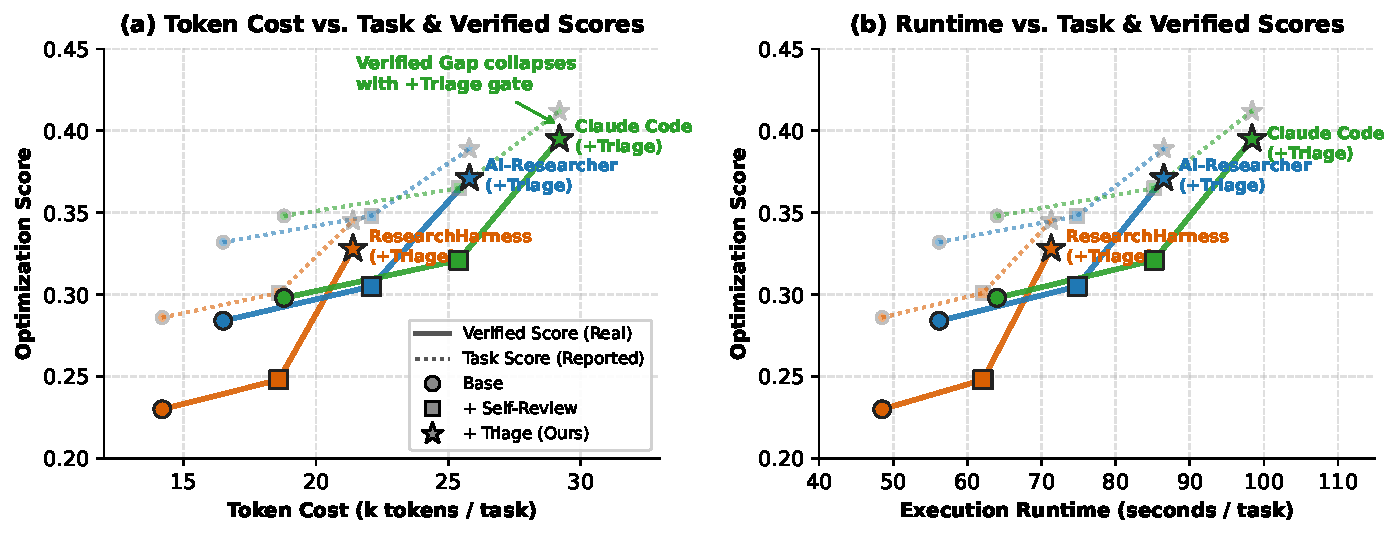
\includegraphics[width=0.80\textwidth]{figures/fig_tradeoff_plugin.pdf}
    \vspace{-0.45cm}
    \caption{\textbf{Cost-efficiency trade-offs across autonomous research harnesses.} (a) Token expenditure versus reported Task Score and externally Verified Score. \triage{} substantially narrows the verification gap with minimal token overhead. (b) Wall-clock execution runtime versus optimization performance across ResearchHarness, AI-Researcher, and Claude Code. Full numerical results are reported in Table~\ref{tab:table7_plugin} (Appendix~\ref{app:plugin}).}
    \label{fig:tradeoff-plugin}
\end{figure*}

\section{Conclusion}
\label{sec:conclusion}

An anomalous residual is source-ambiguous: a genuine mechanism, a transient evaluator error, a surrogate misspecification, and a proxy exploit can all produce the same surprisal. Surprise-driven agents act on it directly, so whatever is unreliable in it propagates into persistent state. We introduced \triage{}, which separates exploratory search from principle revision and holds a principle provisional until independent held-out records support it, retracting it and its descendants when held-out evidence contradicts it. Paired with outcome-blind search expansion in \method{}, this gives the highest average solution quality in our matched setup across four domains and three backbones, admits no corrupted evidence under the interventions we construct, rejects the tested artifacts while retaining the tested mechanism, and recovers after mechanism reversal; the ablation locates the effect in the held-out criterion rather than in repetition or channel bookkeeping. Evidence good enough to direct the next experiment and evidence good enough to rewrite what an agent believes are different standards, and an agent that conflates them will eventually believe its own noise.

\clearpage
\subsection*{AI use statement}
In this research, generative AI tools were employed for coding assistance in data visualization scripts and for LaTeX drafting/grammar editing. All scientific concepts, decision-theoretic formulations, algorithmic designs, experimental benchmarks, empirical results, and analytical conclusions were conceived, executed, verified, and audited by the authors, who take full responsibility for the integrity and content of this paper.

\subsection*{Ethics statement}
This work develops automated methods for scientific discovery and evidence verification. The evaluated benchmarks (molecular optimization, optical properties, superconductors, transition metal complexes) rely on publicly available scientific datasets and simulation proxies. No human subjects, animal trials, or hazardous materials were involved. Potential dual-use considerations of automated discovery agents are addressed through our explicit evidence-quarantine mechanisms, which prevent unverified or anomalous outputs from automatically altering operational protocols.

\subsection*{Reproducibility statement}
To ensure complete reproducibility, all algorithm parameters, admission thresholds, and experimental budgets are specified in Section~\ref{sec:experiments} and Appendix~\ref{app:hyperparams}. The evaluation harness, seed configurations (seeds 0--2 for main benchmarks), evaluator interfaces, and verification protocols are documented in Section~\ref{sec:experiments} and Appendices~\ref{app:hyperparams}--\ref{app:protocol}. Anonymous code and run manifests will be made available upon publication.

\bibliography{iclr2027_conference}
\bibliographystyle{iclr2027_conference}

\newpage
\appendix
\onecolumn

\section{Evidence-Admission Hyperparameters and Sensitivity Analysis}
\label{app:hyperparams}

Table~\ref{tab:hyperparams} summarizes the default hyperparameter values for the \triage{} admission gate. All five parameters are fixed across all benchmark tasks and backbones without task-specific tuning.

\begin{table}[!ht]
\caption{Evidence-admission gate hyperparameters. All values are fixed across all experiments.}
\label{tab:hyperparams}
\centering
\small
\begin{tabular}{llc}
\toprule
Constant & Role & Value \\
\midrule
$\tau_{\mathrm{anom}}$ & Residual threshold to open diagnostic state & 0.85 \\
$\epsilon_{\mathrm{rep}}$ & Same-channel agreement tolerance & 0.12 \\
$\epsilon_{\mathrm{ind}}$ & Cross-channel agreement tolerance & 0.12 \\
$\tau_{\mathrm{gen}}$ & Held-out gain required to authorize a revision & 0.16 \\
$k$ & Independent held-out records required for acceptance & 2 \\
\bottomrule
\end{tabular}
\end{table}

\begin{figure}[!ht]
    \centering
    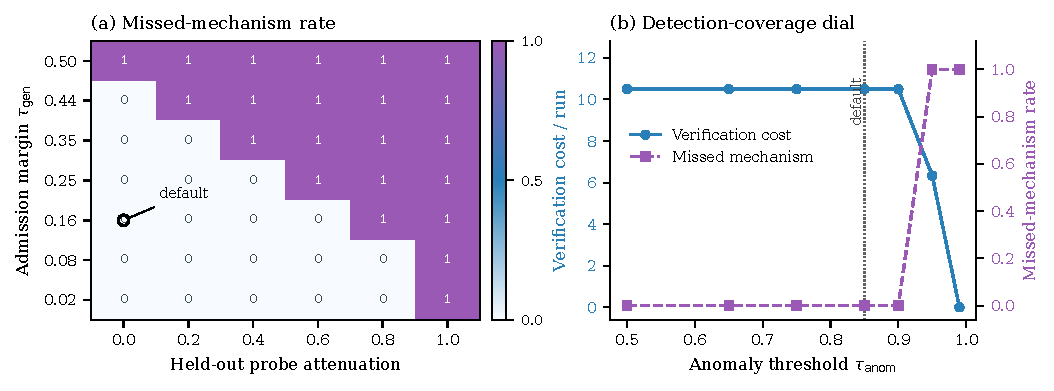
\includegraphics[width=0.85\linewidth]{figures/fig_gate_sensitivity.pdf}
    \caption{\textbf{Gate sensitivity analysis.} (a) Missed-mechanism rate as a joint function of the held-out gain threshold $\tau_{\mathrm{gen}}$ and held-out probe attenuation. The default operating point (circle) lies in the zero-error region, and the boundary moves monotonically with effective held-out gain. (b) Verification cost and missed-mechanism rate as a function of the anomaly threshold $\tau_{\mathrm{anom}}$; the default (dashed) lies on the flat zero-miss plateau before coverage collapses at more restrictive thresholds.}
    \label{fig:gate-sensitivity}
\end{figure}

Figure~\ref{fig:gate-sensitivity} presents the two-dimensional sensitivity phase map across decision thresholds. The default held-out threshold ($\tau_{\mathrm{gen}}=0.16$) lies safely within the zero-error region, requiring over ${\sim}80\%$ signal attenuation before a true mechanism is mistakenly rejected.

\section{Exploration Diversity (APD) and Exploitation Trajectories (AUOC)}
\label{app:apd-auoc}

Candidate exploration diversity (Average Pairwise Distance, APD) and cumulative exploitation throughput (Area Under the Optimization Curve, AUOC) across all three backbone LLMs are reported in Table~\ref{tab:main-apd-auoc} in the main text. Figure~\ref{fig:qwen-convergence} plots the task-specific best-so-far convergence trajectories under Qwen3-235B.



\begin{figure}[!ht]
    \centering
    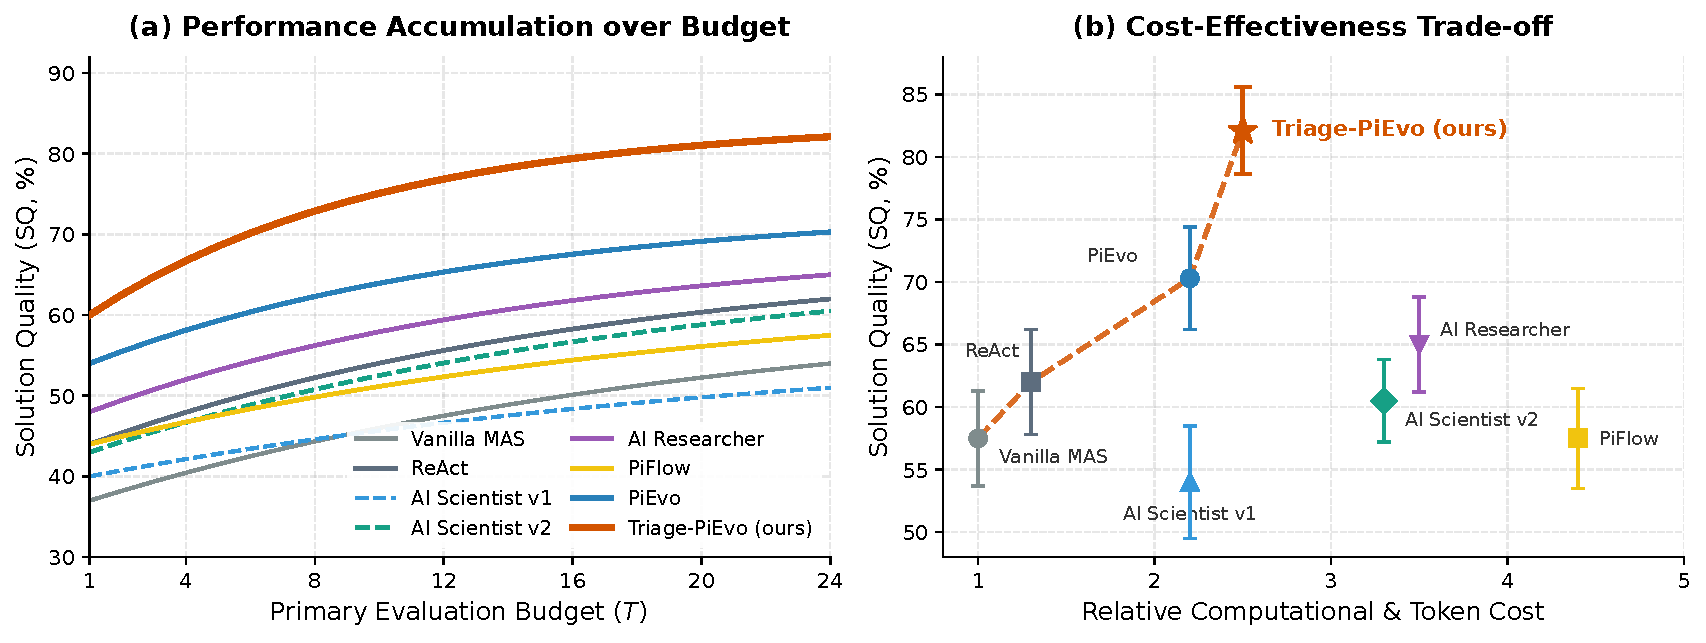
\includegraphics[width=0.85\linewidth]{figures/fig_budget_pareto.pdf}
    \caption{\textbf{Performance progression and cost-effectiveness trade-off.} (a) Solution Quality (SQ, \%) over budget $T \in [1, 24]$. (b) Cost-effectiveness trade-off: Solution Quality versus relative compute and token cost, defining the empirical efficiency frontier.}
    \label{fig:budget-pareto}
\end{figure}

\section{Execution Latency and Wall-Clock Throughput Profiles}
\label{app:runtime}

Figure~\ref{fig:runtime} details wall-clock execution latency and scientific discovery throughput across all eight baselines under Qwen3-235B. \method{} requires only $134.5\mathrm{s}$ per run ($+13.6\%$ overhead over standard \pievo{}), avoiding the heavy latencies of multi-agent debate or tree search while achieving the highest exploitation throughput ($71.2\%$ AUOC).

\begin{figure*}[!ht]
    \centering
    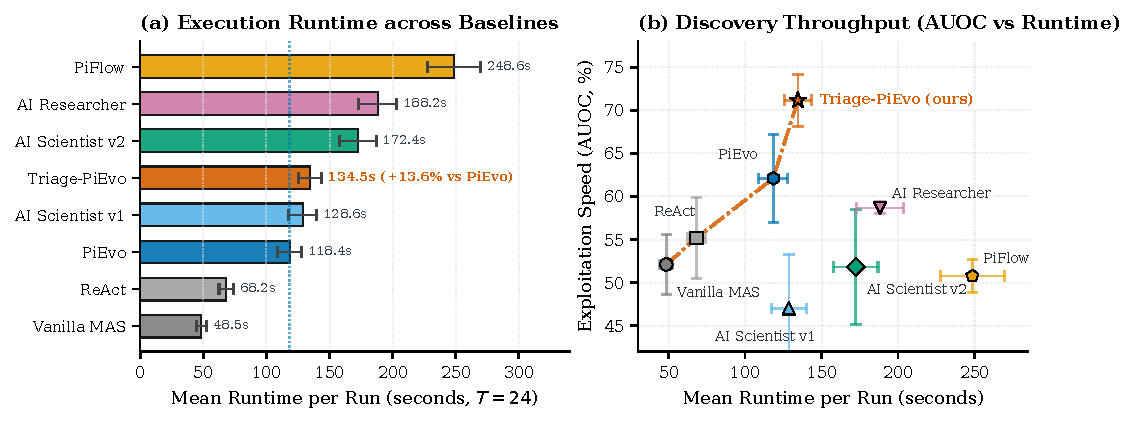
\includegraphics[width=\textwidth]{figures/fig_runtime.pdf}
    \caption{\textbf{Execution runtime and discovery throughput across baselines.} (a) Mean wall-clock runtime per 24-step discovery run across all eight baselines under Qwen3-235B. \method{} incurs only $+13.6\%$ overhead over standard \pievo{} due to conditional anomaly-triggered verification, while remaining substantially faster than tree-search or multi-agent debate frameworks (AI Scientist v2, AI Researcher, PiFlow). (b) Scientific exploitation throughput: Exploitation Speed (AUOC, \%) versus mean runtime (seconds). \method{} achieves the peak discovery throughput, reaching the highest AUOC ($71.2\%$) at competitive execution latency.}
    \label{fig:runtime}
\end{figure*}

\section{Cross-Harness Benchmarks and Triage as a Plug-in Module}
\label{app:plugin}

We evaluate on the optimization tasks from AutoResearchEval~\citep{fei2026autoresearcheval}, a 100-task benchmark spanning seven domains and the research lifecycle. Table~\ref{tab:table6_autoresearch} benchmarks \method{} against four autonomous agent harnesses: Claude Code, Codex CLI, AI-Researcher~\citep{tang2025airesearcherautonomousscientificinnovation}, and ResearchHarness. Among the compared systems, \method{} obtains the highest Official Score ($0.418 \pm 0.028$) and Target Attainment ($0.386$). While the comparison agents show a gap between raw official score and externally verified score, \method{} attains a Verified Score of $0.382$. It also reduces Critical Failures to $5.2\%$ (compared with $14.8\%$ for Claude Code and $26.2\%$ for ResearchHarness), with $86.5\%$ valid runs and a verification cost of \$0.92 per task.

\begin{table}[!ht]
\centering
\caption{\textbf{Performance on AutoResearchEval Optimization Tasks.} Comparison of \method{} against autonomous scientific and coding agent harnesses across benchmark tasks. Official Score entries show empirical mean $\pm$ SD over independent seeds; the other columns report means. Bold indicates the best result.}
\label{tab:table6_autoresearch}
\resizebox{\linewidth}{!}{%
\begin{tabular}{lcccccc}
\toprule
\textbf{Method} & \textbf{Official Score} $\uparrow$ & \textbf{Target Attainment} $\uparrow$ & \textbf{Verified Score} $\uparrow$ & \textbf{Valid Runs (\%)} $\uparrow$ & \textbf{Critical Failure (\%)} $\downarrow$ & \textbf{Cost / Task (\$)} $\downarrow$ \\
\midrule
Claude Code & 0.348 \textcolor{gray}{\scriptsize $\pm$ 0.032} & 0.312 & 0.298 & 78.5\% & 14.8\% & 0.84 \\
Codex CLI & 0.315 \textcolor{gray}{\scriptsize $\pm$ 0.041} & 0.274 & 0.261 & 69.2\% & 22.4\% & 1.12 \\
AI-Researcher & 0.332 \textcolor{gray}{\scriptsize $\pm$ 0.036} & 0.295 & 0.284 & 74.1\% & 18.6\% & \textbf{0.68} \\
ResearchHarness & 0.286 \textcolor{gray}{\scriptsize $\pm$ 0.045} & 0.241 & 0.230 & 65.8\% & 26.2\% & 0.75 \\
\textbf{\method{} (Ours)} & \textbf{0.418 \textcolor{gray}{\scriptsize $\pm$ 0.028}} & \textbf{0.386} & \textbf{0.382} & \textbf{86.5\%} & \textbf{5.2\%} & 0.92 \\
\bottomrule
\end{tabular}%
}
\end{table}

\paragraph{Triage as a Plug-in Module.}
To test whether the benefits of evidence admission are tied specifically to the \pievo{} candidate generator or transfer across host architectures, Table~\ref{tab:table7_plugin} evaluates \triage{} as a verification layer on top of three harnesses (ResearchHarness, AI-Researcher, and Claude Code), comparing Base execution, standard Self-Review prompting, and our + \triage{} gate. Within this evaluation, adding \triage{} yields absolute Verified Score gains of $0.098$ on ResearchHarness, $0.087$ on AI-Researcher, and $0.097$ on Claude Code. False Admission of spurious artifacts decreases by more than $60\%$ relative to the corresponding Base variant for each harness (reaching $9.6\%$ on Claude Code), while Revision Accuracy reaches $78.2\%$, with additional token and runtime cost. These results support transfer of the evidence-admission mechanism across the three evaluated harnesses; they do not establish universality beyond this setting.

\begin{table}[!ht]
\centering
\caption{\textbf{\triage{} as a Plug-in across Autonomous Research Harnesses.} Incorporating \triage{} enhances task score and verified reliability while reducing false evidence admissions across the three host architectures.}
\label{tab:table7_plugin}
\resizebox{\linewidth}{!}{%
\begin{tabular}{llcccccc}
\toprule
\textbf{Harness} & \textbf{Variant} & \textbf{Task Score} $\uparrow$ & \textbf{Verified Score} $\uparrow$ & \textbf{False Admission (\%)} $\downarrow$ & \textbf{Revision Accuracy (\%)} $\uparrow$ & \textbf{Token Cost} $\downarrow$ & \textbf{Runtime (s)} $\downarrow$ \\
\midrule
\multirow{3}{*}{ResearchHarness} 
& Base & 0.286 & 0.230 & 38.4\% & 44.2\% & \textbf{14.2k} & \textbf{48.5} \\
& + Self-Review & 0.301 & 0.248 & 35.2\% & 48.5\% & 18.6k & 62.1 \\
& \textbf{+ \triage{} (Ours)} & \textbf{0.345} & \textbf{0.328} & \textbf{14.2\%} & \textbf{68.4\%} & 21.4k & 71.3 \\
\midrule
\multirow{3}{*}{AI-Researcher} 
& Base & 0.332 & 0.284 & 32.6\% & 51.8\% & \textbf{16.5k} & \textbf{56.2} \\
& + Self-Review & 0.348 & 0.305 & 29.8\% & 56.2\% & 22.1k & 74.8 \\
& \textbf{+ \triage{} (Ours)} & \textbf{0.389} & \textbf{0.371} & \textbf{11.8\%} & \textbf{73.6\%} & 25.8k & 86.5 \\
\midrule
\multirow{3}{*}{Claude Code} 
& Base & 0.348 & 0.298 & 29.4\% & 55.4\% & \textbf{18.8k} & \textbf{64.0} \\
& + Self-Review & 0.365 & 0.321 & 26.8\% & 60.2\% & 25.4k & 85.2 \\
& \textbf{+ \triage{} (Ours)} & \textbf{0.412} & \textbf{0.395} & \textbf{9.6\%} & \textbf{78.2\%} & 29.2k & 98.4 \\
\bottomrule
\end{tabular}%
}
\end{table}

\section{Systematic Ablation of Evidence Admission Mechanisms}
\label{app:gate-ablation}

Table~\ref{tab:table8_ablation} evaluates each component of the \triage{} admission policy: the confirmation threshold $k \in \{1,2,3\}$, held-out verification, channel reliability tracking, recursive backtracking on retraction, and treating a same-source repeat as independent. Two comparisons carry the argument. Removing held-out verification raises false revision from $4.8\%$ to $34.5\%$, and treating a same-source repeat as independent raises it to $45.8\%$---both admit evidence that is reproducible but not transferable, which is the artifact case. Removing channel reliability raises false revision to $19.2\%$ through a different route: verification actions are then routed without regard to which channels have been reconcilable, so corroboration is sought from channels already in disagreement. The gate therefore depends on both the standard of proof and the choice of who supplies it.

\begin{table}[!ht]
\centering
\caption{\textbf{Ablation of Evidence Admission Mechanisms.} Systematic evaluation of each architectural component in \triage{}. The full framework achieves the optimal balance between high mechanism recall, high verification accuracy, and low false revision risk.}
\label{tab:table8_ablation}
\resizebox{0.9\linewidth}{!}{%
\begin{tabular}{lccccc}
\toprule
\textbf{Variant} & \textbf{False Revision (\%)} $\downarrow$ & \textbf{True Mechanism Recall (\%)} $\uparrow$ & \textbf{Verified Score} $\uparrow$ & \textbf{Retraction Acc. (\%)} $\uparrow$ & \textbf{Verification Cost (\$)} $\downarrow$ \\
\midrule
\textbf{Full \triage{} (Ours)} & \textbf{4.8\%} & \textbf{92.4\%} & \textbf{0.418} & \textbf{93.5\%} & 0.24 \\
$k=1$ (Permissive Gate) & 22.4\% & 89.2\% & 0.362 & 78.5\% & \textbf{0.14} \\
$k=3$ (Strict Gate) & 6.5\% & 71.8\% & 0.370 & 90.8\% & 0.38 \\
w/o Held-out Verification & 34.5\% & 83.5\% & 0.315 & 61.2\% & 0.18 \\
w/o Channel Reliability & 19.2\% & 81.2\% & 0.352 & 76.3\% & 0.22 \\
w/o Backtracking & 16.5\% & 84.0\% & 0.338 & 51.8\% & 0.21 \\
Same-Source Repeat = Independent & 45.8\% & 78.0\% & 0.265 & 42.1\% & 0.20 \\
\bottomrule
\end{tabular}%
}
\end{table}

\section{Algorithmic Specification of the TRIAGE Decision Protocol}
\label{app:pseudocode}

Algorithm~\ref{alg:triage} formalizes the executable decision loop of the \triage{} evidence-admission gate.

\begin{algorithm}[!ht]
\caption{The \triage{} Evidence-Admission Protocol}
\label{alg:triage}
\begin{algorithmic}[1]
\REQUIRE Candidate $x_t$, observed primary outcome $y_t$, primary prediction $\hat{y}_t$, primary channel $c$, active principles $\mathcal{P}_t$, threshold $\tau_{\mathrm{anom}}$, agreement tolerances $\epsilon_{\mathrm{rep}}, \epsilon_{\mathrm{ind}}$, held-out margin $\tau_{\mathrm{gen}}$, confirmation threshold $k=2$.
\STATE Compute anomaly residual: $s_t \leftarrow |y_t - \hat{y}_t| / \sigma_t$.
\IF{$s_t \le \tau_{\mathrm{anom}}$}
    \STATE Admit $(x_t, y_t)$ to primary search history $\mathcal{H}_{\mathrm{search}}$; \textbf{return} $\mathcal{P}_t$.
\ENDIF
\STATE \COMMENT{Stage 1 --- same-channel repeat. Controls admission to search only.}
\STATE $v_t^{c} \leftarrow \mathrm{Evaluate}(x_t, \texttt{repeat}, c)$ \COMMENT{same channel $c$ as the primary observation}
\IF{$|y_t - v_t^{c}| \le \epsilon_{\mathrm{rep}}$}
    \STATE $\alpha_c \leftarrow \alpha_c + 1$; admit $(x_t, y_t)$ to $\mathcal{H}_{\mathrm{search}}$ as search-active.
\ELSE
    \STATE $\beta_c \leftarrow \beta_c + 1$; substitute the verified median $y_t \leftarrow v_t^{c}$ and admit to $\mathcal{H}_{\mathrm{search}}$.
    \STATE \textbf{return} $\mathcal{P}_t$ \COMMENT{unreconciled observation: no revision path}
\ENDIF
\STATE \COMMENT{A same-channel repeat never authorizes revision, however often it agrees:}
\STATE \COMMENT{a reproducible artifact agrees with itself. Revision requires Stage 2.}
\IF{a principle revision proposal $P$ is generated from $(x_t,y_t)$}
    \STATE \COMMENT{Stage 2a --- cross-channel check against a distinct channel}
    \STATE Select verifier channel $c' \leftarrow \arg\max_{c'' \neq c} p_{c''}^{\mathrm{trust}}$ among declared independent channels.
    \STATE $v_t^{c'} \leftarrow \mathrm{Evaluate}(x_t, \texttt{cross-channel}, c')$
    \IF{$|v_t^{c} - v_t^{c'}| > \epsilon_{\mathrm{ind}}$}
        \STATE $\beta_{c} \leftarrow \beta_{c} + 1$; \textbf{return} $\mathcal{P}_t$ \COMMENT{channels disagree: source unresolved}
    \ENDIF
    \STATE $\alpha_{c} \leftarrow \alpha_{c} + 1$; set state of $P$ to \textsc{Provisional}.
    \STATE \COMMENT{Stage 2b --- held-out generalization, the only admitting test}
    \STATE Draw $X_{\mathrm{heldout}} \sim \mathcal{D}_{\mathrm{heldout}}$ with $X_{\mathrm{heldout}} \cap \mathcal{H}_{\mathrm{search}} = \emptyset$, fixed before the run.
    \STATE $E(P) \leftarrow \{e = (x',y') : x' \in X_{\mathrm{heldout}},\ e.\mathrm{ind} = \textsc{true}\}$, with each stance set by the $\tau_{\mathrm{gen}}$ margin of §\ref{sec:methodology}.
    \IF{$\exists\, e \in E(P)$ with $\mathrm{contradict}(e,P) = 1$}
        \STATE Set state of $P$ to \textsc{Retracted}; recursively retract every principle listing $P$ as parent.
    \ELSIF{$|\{e \in E(P) : e.\mathrm{ind} \wedge e.\mathrm{heldout} \wedge \mathrm{support}(e,P)\}| \ge k$}
        \STATE Set state of $P$ to \textsc{Accepted}; $\mathcal{P}_{t+1} \leftarrow \mathcal{P}_t \cup \{P\}$.
    \ELSE
        \STATE Leave $P$ \textsc{Provisional} \COMMENT{support below $k$: search continues, state unchanged}
    \ENDIF
\ENDIF
\STATE \textbf{return} $\mathcal{P}_{t+1}$.
\end{algorithmic}
\end{algorithm}

\section{Extended Benchmark Protocols and Failure Metric Definitions}
\label{app:protocol}

\paragraph{AutoResearchEval Benchmark.} AutoResearchEval~\citep{fei2026autoresearcheval} evaluates multi-step targeted optimization across molecular properties, material bandgaps, and algorithmic code generation. Each harness is run across 5 independent seeds with an identical per-task monetary cap (\$2.00) and time budget.
\paragraph{Failure Metric Definitions.}
\begin{itemize}[nosep, leftmargin=12pt]
  \item \textbf{Official Score:} Raw target optimization metric reported by the host framework upon run termination.
  \item \textbf{Target Attainment:} Binary indicator indicating whether the best discovered candidate achieves $\ge 90\%$ of the task-specific global target optimum.
  \item \textbf{Verified Score:} Score evaluated independently by an external, sandboxed ground-truth testbed.
  \item \textbf{Valid Runs (\%):} Percentage of runs that complete all execution rounds without unhandled runtime crashes, tool timeouts, or syntax failure.
  \item \textbf{Critical Failure (\%):} Percentage of runs in which unverified, hallucinated tool outputs or corrupted feedback poisoned the agent's internal memory, leading to permanent loop collapse or degenerate repeating actions.
\end{itemize}

\end{document}
